% !TEX option = -shell-escape

% \newcommand{\compacttitlespacing}{0} %disable when we need room for authors
\documentclass[sigconf, review]{acmart}
\newcommand{\sub}[2]{\text{#1}_{\text{#2}}}
\settopmatter{printacmref=false}
\renewcommand\footnotetextcopyrightpermission[1]{}
\setcopyright{none}
% defining the \BibTeX command - from Oren Patashnik's original BibTeX documentation.
\def\BibTeX{{\rm B\kern-.05em{\sc i\kern-.025em b}\kern-.08emT\kern-.1667em\lower.7ex\hbox{ E}\kern-.125emX}}
\usepackage{nicefrac}
\usepackage{siunitx}
\usepackage{tabularx}
\usepackage{minted}
\usepackage{svg}
\usepackage{url}
\usepackage{array,framed}
\usepackage{booktabs}
\usepackage{
  color,
  float,
  epsfig,
  wrapfig,
  graphics,
  graphicx,
  subcaption
}
% \usepackage[dvipsnames]{xcolor}
\let\Bbbk\relax
\usepackage{textcomp,amssymb}
\usepackage{setspace}
% \usepackage{amsfonts}
\usepackage{latexsym,fancyhdr,url}
\usepackage{enumerate}
\usepackage{algorithm2e}
\usepackage{algpseudocode}
\usepackage{graphics}
\usepackage{xparse} % argument parsing -- \edist
\usepackage{xspace}
\usepackage{multirow}
\usepackage{csvsimple}
\usepackage{balance}
% \usepackage{flushend}
% \usepackage{mathptmx,avant}
\usepackage{caption}
\captionsetup{skip=10pt}

%%%% Tikz variables, pgfplot
\usepackage{
  tikz,
  pgfplots,
  pgfplotstable
}
\usepackage{hyperref}

\usetikzlibrary{
  shapes.geometric,
  arrows,
  external,
  pgfplots.groupplots,
  matrix
}

\pgfplotsset{compat=1.9}
% \tikzexternalize[prefix=images/]
% \tikzexternalenable

%\pagenumbering{arabic}
% \pagestyle{plain}

\usepackage{mathtools,}
\DeclarePairedDelimiter\abs{\lvert}{\rvert}
\DeclarePairedDelimiter\norm{\lVert}{\rVert}

% \setmathfont{Latin Modern Math}[version=lm]
\DeclareMathAlphabet{\mathcal}{OMS}{cmsy}{m}{n}
% \DeclareSymbolFont{operators}{T1}{cmr}{m}{n}
% \DeclareSymbolFont{letters}{OML}{cmm}{m}{it}
% \DeclareSymbolFont{symbols}{OMS}{cmsy}{m}{n}
% \DeclareSymbolFont{largesymbols}{OMX}{cmex}{m}{n}

% \usepackage{times}

% \setmathcal{Arial}

% TO deal with the weird flow of boxes
% \brokenpenalty=1000
% \clubpenalty=1000
% \widowpenalty=10
\DeclareGraphicsExtensions{%
    .png,.PNG,%
    .pdf,.PDF,%
    .jpg,.mps,.jpeg,.jbig2,.jb2,.JPG,.JPEG,.JBIG2,.JB2}

\usepackage{xparse}
\newcommand{\bnm}{\begin{newmath}}
\newcommand{\enm}{\end{newmath}}

\newcommand{\bea}{\begin{eqnarray*}}%
\newcommand{\eea}{\end{eqnarray*}}%

\newcommand{\bne}{\begin{newequation}}
\newcommand{\ene}{\end{newequation}}

\newcommand{\bal}{\begin{newalign}}
\newcommand{\eal}{\end{newalign}}

\newenvironment{newalign}{\begin{align}%
\setlength{\abovedisplayskip}{4pt}%
\setlength{\belowdisplayskip}{4pt}%
\setlength{\abovedisplayshortskip}{6pt}%
\setlength{\belowdisplayshortskip}{6pt} }{\end{align}}

\newenvironment{newmath}{\begin{displaymath}%
\setlength{\abovedisplayskip}{4pt}%
\setlength{\belowdisplayskip}{4pt}%
\setlength{\abovedisplayshortskip}{6pt}%
\setlength{\belowdisplayshortskip}{6pt} }{\end{displaymath}}

\newenvironment{neweqnarrays}{\begin{eqnarray*}%
\setlength{\abovedisplayskip}{-4pt}%
\setlength{\belowdisplayskip}{-4pt}%
\setlength{\abovedisplayshortskip}{-4pt}%
\setlength{\belowdisplayshortskip}{-4pt}%
\setlength{\jot}{-0.4in} }{\end{eqnarray*}}

\newenvironment{newequation}{\begin{equation}%
\setlength{\abovedisplayskip}{4pt}%
\setlength{\belowdisplayskip}{4pt}%
\setlength{\abovedisplayshortskip}{6pt}%
\setlength{\belowdisplayshortskip}{6pt} }{\end{equation}}


\newcounter{ctr}
\newcounter{savectr}
\newcounter{ectr}

\newenvironment{newitemize}{%
\begin{list}{\mbox{}\hspace{5pt}$\bullet$\hfill}{\labelwidth=15pt%
\labelsep=4pt \leftmargin=12pt \topsep=3pt%
\setlength{\listparindent}{\saveparindent}%
\setlength{\parsep}{\saveparskip}%
\setlength{\itemsep}{3pt} }}{\end{list}}


\newenvironment{newenum}{%
\begin{list}{{\rm (\arabic{ctr})}\hfill}{\usecounter{ctr} \labelwidth=17pt%
\labelsep=5pt \leftmargin=22pt \topsep=3pt%
\setlength{\listparindent}{\saveparindent}%
\setlength{\parsep}{\saveparskip}%
\setlength{\itemsep}{2pt} }}{\end{list}}

%%%%%%%%%%%%%%%%%%%%%%%%%%%%%%%%%%%%%%%%%%%%%%%%%%%%%%%%%%%%%%%%%%%%%%%%%%%%%%
%
% Figure and table macros
%

\newcounter{mytable}
\def\mytable{\begin{centering}\refstepcounter{mytable}}
\def\endmytable{\end{centering}}

\def\mytablecaption#1{\vspace{2mm}
  \centerline{Table \arabic{mytable}.~{#1}}
  \vspace{6mm}
  \addcontentsline{lot}{table}{\protect\numberline{\arabic{mytable}}~{#1}}
}


\newcounter{myfig}
\def\myfig{\begin{centering}\refstepcounter{myfig}}
\def\endmyfig{\end{centering}}

\def\myfigcaption#1{
             \vspace{2mm}
             \centerline{\textsf{Figure \arabic{myfig}.~{#1}}}
             \vspace{6mm}
             \addcontentsline{lof}{figure}{\protect\numberline{\arabic{myfig}}~{#1}}}


\newlength{\saveparindent}
\setlength{\saveparindent}{\parindent}
\newlength{\saveparskip}
\setlength{\saveparskip}{\parskip}

\newcommand{\decOracle}{\textbf{Dec}}

\newcommand{\negsmidge}{{\hspace{-0.1ex}}}
\newcommand{\cdotsm}{\negsmidge\negsmidge\negsmidge\cdot\negsmidge\negsmidge\negsmidge}

\def\suchthatt{\: :\:}
\newcommand{\E}{{\rm I\kern-.3em E}}
\newcommand{\Prob}[1]{{\Pr\left[\,{#1}\,\right]}}
\newcommand{\Probb}[2]{{\Pr}_{#1}\left[\,{#2}\,\right]}
\newcommand{\CondProb}[2]{{\Pr}\left[\: #1\:\left|\right.\:#2\:\right]}
\newcommand{\CondProbb}[2]{\Pr[#1|#2]}
\newcommand{\ProbExp}[2]{{\Pr}\left[\: #1\:\suchthatt\:#2\:\right]}
\newcommand{\Ex}[1]{{\textnormal{E}\left[\,{#1}\,\right]}}
\newcommand{\Exx}{{\textnormal{E}}}
\newcommand{\given}{\ensuremath{\,\big|\,}}


\newcommand{\true}{\mathsf{true}}
\newcommand{\false}{\mathsf{false}}
\def\negl{\mathsf{negl}}


\newcommand{\secref}[1]{\mbox{Section~\ref{#1}}}
\newcommand{\appref}[1]{\mbox{Appendix~\ref{#1}}}
\newcommand{\thref}[1]{\mbox{Theorem~\ref{#1}}}
\newcommand{\defref}[1]{\mbox{Definition~\ref{#1}}}
\newcommand{\corref}[1]{\mbox{Corollary~\ref{#1}}}
\newcommand{\lemref}[1]{\mbox{Lemma~\ref{#1}}}
\newcommand{\clref}[1]{\mbox{Claim~\ref{#1}}}
\newcommand{\propref}[1]{\mbox{Proposition~\ref{#1}}}
\newcommand{\factref}[1]{\mbox{Fact~\ref{#1}}}
\newcommand{\remref}[1]{\mbox{Remark~\ref{#1}}}
\newcommand{\figref}[1]{\mbox{Figure~\ref{#1}}}
\renewcommand{\algref}[1]{\mbox{Algorithm~\ref{#1}}}
% \newcommand{\eqref}[1]{\mbox{Equation~(\ref{#1})}}
% Have to use \renewcommand because exists already in amsmath
\renewcommand{\eqref}[1]{\mbox{Equation~(\ref{#1})}}
\newcommand{\consref}[1]{\mbox{Construction~\ref{#1}}}
\newcommand{\tabref}[1]{\mbox{Table~\ref{#1}}}

\newcommand{\get}{{\:{\leftarrow}\:}}
\newcommand{\gett}[1]{\:{\leftarrow}_{#1}\:}
\newcommand{\getsr}{{\:{\leftarrow{\hspace*{-3pt}\raisebox{.75pt}{$\scriptscriptstyle\$$}}}\:}}
\newcommand{\getm}{{\:\leftarrow_{\mdist}\:}}
\newcommand{\getd}{{\:\leftarrow_{\ddist}\:}}
%\newcommand{\getm}{{\:{\leftarrow{\hspace*{-3pt}\raisebox{.75pt}{$\scriptscriptstyle \mdist$}}}\:}}
\newcommand{\getk}{{\:\leftarrow_{\kdist}\:}}
%\newcommand{\getk}{{\:{\leftarrow{\hspace*{-3pt}\raisebox{.75pt}{$\scriptscriptstyle \kdist$}}}\:}}
\newcommand{\getp}{{\:\leftarrow_{p}\:}}



\newcommand{\gamesfontsize}{\small}
\newcommand{\fpage}[2]{\framebox{\begin{minipage}[t]{#1\textwidth}\setstretch{1.1}\gamesfontsize  #2 \end{minipage}}}
\newcommand{\mpage}[2]{\begin{minipage}[t]{#1\textwidth}\setstretch{1.1}\gamesfontsize  #2 \end{minipage}}

\newcommand{\hpages}[3]{\begin{tabular}{cc}\begin{minipage}[t]{#1\textwidth} #2 \end{minipage} & \begin{minipage}[t]{#1\textwidth} #3 \end{minipage}\end{tabular}}

\newcommand{\hpagess}[4]{
        \begin{tabular}[t]{c@{\hspace*{.5em}}c}
        \begin{minipage}[t]{#1\textwidth}\gamesfontsize #3 \end{minipage}
        &
        \begin{minipage}[t]{#2\textwidth}\gamesfontsize #4 \end{minipage}
        \end{tabular}
    }

\newcommand{\hpagesss}[6]{
        \begin{tabular}[t]{c@{\hspace*{.5em}}c@{\hspace*{.5em}}c@{\hspace*{.5em}}c}
        \begin{minipage}[t]{#1\textwidth}\gamesfontsize #4 \end{minipage}
        &
        \begin{minipage}[t]{#2\textwidth}\gamesfontsize #5 \end{minipage}
        &
        \begin{minipage}[t]{#3\textwidth}\gamesfontsize #6 \end{minipage}
        \end{tabular}
    }

\newcommand{\hpagessss}[8]{
        \begin{tabular}{c@{\hspace*{.5em}}c@{\hspace*{.5em}}c@{\hspace*{.5em}}c}
        \begin{minipage}[t]{#1\textwidth}\gamesfontsize #5 \end{minipage}
        &
        \begin{minipage}[t]{#2\textwidth}\gamesfontsize #6 \end{minipage}
        &
        \begin{minipage}[t]{#3\textwidth}\gamesfontsize #7 \end{minipage}
        &
        \begin{minipage}[t]{#4\textwidth}\gamesfontsize #8 \end{minipage}
        \end{tabular}
    }


\newcommand{\hfpages}[3]{\hfpagess{#1}{#1}{#2}{#3}}
\newcommand{\hfpagess}[4]{
        \begin{tabular}[t]{c@{\hspace*{.5em}}c}
        \framebox{\begin{minipage}[t]{#1\textwidth}\setstretch{1.1}\gamesfontsize #3 \end{minipage}}
        &
        \framebox{\begin{minipage}[t]{#2\textwidth}\setstretch{1.1}\gamesfontsize #4 \end{minipage}}
        \end{tabular}
    }
\newcommand{\hfpagesss}[6]{
        \begin{tabular}[t]{c@{\hspace*{.5em}}c@{\hspace*{.5em}}c}
        \framebox{\begin{minipage}[t]{#1\textwidth}\setstretch{1.1}\gamesfontsize #4 \end{minipage}}
        &
        \framebox{\begin{minipage}[t]{#2\textwidth}\setstretch{1.1}\gamesfontsize #5 \end{minipage}}
        &
        \framebox{\begin{minipage}[t]{#3\textwidth}\setstretch{1.1}\gamesfontsize #6 \end{minipage}}
        \end{tabular}
    }
\newcommand{\hfpagessss}[8]{
        \begin{tabular}[t]{c@{\hspace*{.5em}}c@{\hspace*{.5em}}c@{\hspace*{.5em}}c}
        \framebox{\begin{minipage}[t]{#1\textwidth}\setstretch{1.1}\gamesfontsize #5 \end{minipage}}
        &
        \framebox{\begin{minipage}[t]{#2\textwidth}\setstretch{1.1}\gamesfontsize #6 \end{minipage}}
        &
        \framebox{\begin{minipage}[t]{#3\textwidth}\setstretch{1.1}\gamesfontsize #7 \end{minipage}}
        &
        \framebox{\begin{minipage}[t]{#4\textwidth}\setstretch{1.1}\gamesfontsize #8 \end{minipage}}
        \end{tabular}
    }

\newcommand{\vecw}{\mathbf{w}}
\newcommand{\R}{\mathbb{R}}
\newcommand{\N}{\mathbb{N}}
\newcommand{\Z}{\mathbb{Z}}
\newcommand{\load}{L}
\newcommand{\coll}{\mathsf{Coll}}
\newcommand{\nocoll}{\overline{\mathsf{Coll}}}


\newcommand{\Img}{\textsf{Img}}

%%%%%%%%%%%%%%%%%%%%%%%%%%%%%%%%%%%%%%%%%%%%%%%%%%%%%%%%%%%%%%%%%%%%%%%%%%%%%%%%
%%%% Fonts and symbols
%%%%%%%%%%%%%%%%%%%%%%%%%%%%%%%%%%%%%%%%%%%%%%%%%%%%%%%%%%%%%%%%%%%%%%%%%%%%%%%%
\newcommand\funcfont{\textsf}
\newcommand\variablefont{\texttt}

%%%%%%%%%%%%%%%%%%%%%%%%%%%%%%%%%%%%%%%%%%%%%%%%%%%%%%%%%%%%%%%%%%%%%%%%%%%%%%%%
%%%%%%%%%%%%%%%%%%%%%%%%%%%%%%%% NEW COMMANDS %%%%%%%%%%%%%%%%%%%%%%%%%%%%%%%%%%
%%%%%%%%%%%%%%%%%%%%%%%%%%%%%%%%%%%%%%%%%%%%%%%%%%%%%%%%%%%%%%%%%%%%%%%%%%%%%%%%

\def \Perm {\funcfont{Perm}}
\def \calC {{\mathcal{C}}}
\def \calU {{\mathcal{U}}}
\renewcommand{\u}{\ensuremath{u}}
\newcommand{\unew}{\ensuremath{\tilde{u}}}

\newcommand{\calN}{\mathcal{N}}
\def \sspace {{\mathcal{S}}}
\def \strings {{\mathcal{S}}}
\def \slen {{s}}
\def \kspace {{\mathcal{K}}}
\def \kspacesize {{m}}
\def \mspacesize {{n}}
\def \kdict {D}
\def \dictsize {d}
\newcommand{\kdist}{p_k}
\newcommand{\mdist}{\ensuremath{{W}}}
\newcommand{\alldist}{\rho}
\newcommand{\pwdist}{\transgen}
\newcommand{\ddist}{\rho_{dec}}
\newcommand{\PWset}{{\mathcal{P}}}  % TODO: fix, same as \pwdist
\newcommand{\PWsetvec}{\vec{\mathcal{P}}}
\newcommand{\PWvec}{\vec{P}}
\newcommand{\domvec}{\vec{D}}
\newcommand{\humanornot}{\vec{h}}
\newcommand{\dom}{\textsf{dom}}
%\def \kdist {{\kappa}}
%\def \mdist {{\mu}}
%\def \ddist {{\delta}}
\def \pspace {{\mathcal{P}}}
\def \mpspace {{\mathcal{MP}}}
\def \cspace {{\mathcal{C}}}
\def \key {\kappa}
\def \msg {M}
\def \seed {S}
\def \ctxt {C}
\def \ctxtpart {C_2}
\newcommand{\genprime}{{\textsf{GenPrime}}}
\newcommand{\isprime}{{\textsf{IsPrime}}}
\newcommand{\LeastLesserPrime}{{\textsf{PrevPrime}}}
\newcommand{\pwset}{\mathcal{S}}
\newcommand{\DTE}{{\textsf{DTE}}}
\newcommand{\encode}{{\textsf{encode}}}
\newcommand{\decode}{{\textsf{decode}}}

\newcommand{\DTEsingle}{{\textsf{1PW-DTE}}}
\newcommand{\encodesingle}{{\textsf{1PW-encode}}}
\newcommand{\decodesingle}{{\textsf{1PW-decode}}}

\newcommand{\DTErss}{{\textsf{RSS-DTE}}}
\newcommand{\encoderss}{{\textsf{RSS-encode}}}
\newcommand{\decoderss}{{\textsf{RSS-decode}}}

\newcommand{\DTEindep}{{\textsf{MPW-DTE}}}
\newcommand{\encodeindep}{{\textsf{MPW-encode}}}
\newcommand{\decodeindep}{{\textsf{MPW-decode}}}


\newcommand{\DTEsub}{{\textsf{SG-DTE}}}
\newcommand{\encodesub}{{\textsf{SG-encode}}}
\newcommand{\decodesub}{{\textsf{SG-decode}}}
\newcommand{\decodekamf}{{\textsf{KAMF-decode}}}
\newcommand{\DTEis}{{\textsf{IS-DTE}}}
\newcommand{\encodeis}{{\textsf{is-encode}}}
\newcommand{\decodeis}{{\textsf{is-decode}}}
\newcommand{\DTErej}{{\textsf{REJ-DTE}}}
\newcommand{\encoderej}{{\textsf{rej-encode}}}
\newcommand{\decoderej}{{\textsf{rej-decode}}}
\newcommand{\DTErsarej}{{\textsf{RSA-REJ-DTE}}}
\newcommand{\encodeRSAREJ}{{\textsf{rsa-rej-encode}}}
\newcommand{\decodeRSAREJ}{{\textsf{rsa-rej-decode}}}
\newcommand{\DTErsainc}{{\textsf{RSA-INC-DTE}}}
\newcommand{\encodeRSAINC}{{\textsf{rsa-inc-encode}}}
\newcommand{\decodeRSAINC}{{\textsf{rsa-inc-decode}}}
\newcommand{\DTEunf}{{\textsf{UNF-DTE}}}
\newcommand{\DTEnunf}{{\textsf{NUNF-DTE}}}


%\newcommand{\encodeis}{{\textsf{encode}_{\textrm{is}}}}
%\newcommand{\decodeis}{{\textsf{decode}_{\textrm{is}}}}
\newcommand{\rep}{\textsf{rep}}
\newcommand{\isErr}{\epsilon_{\textnormal{is}}}
\newcommand{\incErr}{\epsilon_{\textnormal{inc}}}
\def \enc {{\textsf{E}}}
\def \dec {{\textsf{D}}}
\def \SEscheme {{\textsf{SE}}}
\def \HEscheme {{\textsf{HE}}}
\def \CTR {{\textsf{CTR}}}
\def \encHE {{\textsf{HEnc}}}
\def \HIDE {{\textsf{HiaL}}}
\def \encHIDE {{\textsf{HEnc}}}
\def \decHIDE {{\textsf{HDec}}}
\def \decHE {{\textsf{HDec}}}
\def \encHEt {{\textsf{HEnc2}}}
\def \decHEt {{\textsf{HDec2}}}

\newcommand{\myind}{\hspace*{1em}}
\newcommand{\thh}{^{\textit{th}}} % th
\newcommand{\concat}{\,\|\,}
\newcommand{\dotdot}{..}
\newcommand{\emptystr}{\varepsilon}

\newcommand{\round}{\textsf{round}}

\newcommand{\alphabar}{\overline{\alpha}}
\newcommand{\numbinsbar}{\overline{b}}
\newcommand{\numballs}{a}
\newcommand{\numbins}{b}

%\def \encHE {{\sf{enc}^{HE}}}
%\def \decHE {{\sf{dec}^{HE}}}
%\def \encHEt {{\sf{enc}^{HE2}}}
%\def \decHEt {{\sf{dec}^{HE2}}}
\def \idealHE {{\mathcal{HE}}}
\def \IEnc {{\mathbf{\rho}}}
\def \IDec {{\mathbf{\rho^{-1}}}}
\def \OEnc {{\mathbf{Enc}}}
\def \ODec {{\mathbf{Dec}}}
\newcommand{\SimuProc}{\mathbf{Sim}}
\newcommand{\ROProc}{\mathbf{RO}}
\newcommand{\PrimProc}{\mathbf{Prim}}
\def \stm {g}
\def \istm {\hat{g}}
\def \kts {{f}}
\def \lex {{\sf lex}}
\def \part {part}
\def \kd {{\sf{kd}}}
\def \msgdist {{d}}
\def \keydist {{r}}
\def \ind {{\sf{index}}}
\def \kprf {z}
\def \adv {{\mathcal A}}
\def \pwds {u}
\newcommand{\mpw}{mpw}
\newcommand{\pw}{w}
\newcommand{\pwvec}{\vec{\pw}}
\newcommand{\vecx}{\vec{x}}
\def \tokens {v}
\def \calP{{\mathcal{P}}}
\def \template{{\mathcal{T}}}
\def \vaultset{{\mathcal{V}}}
\def \ext {{\sf ext}}
\def \offset {\delta}
\def \maxweight {\epsilon}
\def \advo {{\mathcal{A}}^{*}}

\newcommand{\Chall}{\textsf{Ch}}
\newcommand{\Test}{\textnormal{\textsf{Test}}}
\newcommand{\RoR}{\textsf{RoR}}
\newcommand{\MI}{\textnormal{MI}}
\providecommand{\MR}{\textnormal{MR}}
\newcommand{\MRCCA}{\textnormal{MR-CCA}}
\newcommand{\SAMP}{\textnormal{SAMP}}
\newcommand{\DTEgame}{\textnormal{SAMP}}
\newcommand{\KR}{\textnormal{KR}}
\newcommand{\advA}{{\mathcal{A}}}
\newcommand{\advR}{{\mathcal{R}}}
\newcommand{\advB}{{\mathcal{B}}} % 
\newcommand{\advC}{{\mathcal{C}}} % C
\newcommand{\advD}{{\mathcal{D}}} % D
\newcommand{\advE}{{\mathcal{E}}}
\newcommand{\advF}{{\mathcal{F}}}
\newcommand{\advG}{{\mathcal{G}}}
\newcommand{\advI}{{\mathcal{I}}}
\newcommand{\nextval}{\;;\;}
\newcommand{\TabC}{\texttt{C}}
\newcommand{\TabR}{\texttt{R}}
\newcommand{\Hash}{H}
\newcommand{\Cipher}{\pi}
\newcommand{\CipherInv}{\pi^{-1}}
\newcommand{\simu}{{\mathcal S}}
\newcommand{\prim}{P}
\newcommand{\maxguess}{\gamma}


\newcommand{\bigO}{\mathcal{O}}
\newcommand{\calG}{{\mathcal{G}}}

\def\sqed{{\hspace{5pt}\rule[-1pt]{3pt}{9pt}}}
\def\qedsym{\hspace{2pt}\rule[-1pt]{3pt}{9pt}}

\newcommand{\Colon}{{\::\;}}
\newcommand{\good}{\textsf{Good}}

\newcommand\Tvsp{\rule{0pt}{2.6ex}}
\newcommand\Bvsp{\rule[-1.2ex]{0pt}{0pt}}
\newcommand{\TabPad}{\hspace*{5pt}}
\newcommand\TabSep{@{\hspace{5pt}}|@{\hspace{5pt}}}
\newcommand\TabSepLeft{|@{\hspace{5pt}}}
\newcommand\TabSepRight{@{\hspace{5pt}}|}


\DeclareMathOperator*{\argmin}{argmin}
\DeclareMathOperator*{\argmax}{argmax}
\newcommand{\comma}{\textnormal{,}}

\renewcommand{\paragraph}[1]{\vspace*{6pt}\noindent\textbf{#1}\;}

\newcommand{\weirvault}{\textsf{Pastebin}\xspace}
\newcommand{\ndssvault}{\textsf{DBCBW}\xspace}




\newcommand{\reminder}[1]{ [[[ \marginpar{\mbox{$<==$}} #1 ]]] }

%
% New theorem types: (Already in CCS template)
%
\newtheorem{observation}{Observation}
%\newtheorem{definition}{Definition}
\newtheorem{claim}{Claim}
\newtheorem{assumption}{Assumption}
\newtheorem{fact}{Fact}
% \newtheorem{theorem}{Theorem}[section]
% \newtheorem{lemma}{Lemma}[section]
% \newtheorem{corollary}{Corollary}[section]
% \newtheorem{proposition}{Proposition}
% \newtheorem{example}{Example}

%
% Definitions:
%
\def \blackslug{\hbox{\hskip 1pt \vrule width 4pt height 8pt
    depth 1.5pt \hskip 1pt}}
\def \qed{\quad\blackslug\lower 8.5pt\null\par}
% In-line QED, for ending a proof with a $$ formula
% In-line QED, for ending a proof with a $$ formula
\def \inQED{\quad\quad\blackslug}
\def \Qed{\QED}
\def \QUAD{$\Box$}
\def \Proof{\par\noindent{\bf Proof:~}}
\def \proof{\Proof}
\def \poly {\mbox{$\mathsf{poly}$}}
\def \binary {\mbox{$\mathsf{binary}$}}
\def \ones {\mbox{$\mathsf{ones}$}}
\def \rank {\mbox{$\mathsf{rank}$}}
\def \bits {\mbox{$\mathsf{bits}$}}
\def \factorial {\mbox{$\mathsf{factorial}$}}
\def \fr {\mbox{$\mathsf{fr}$}}
\def \pr {\mbox{$\mathsf{pr}$}}
\def \zon {\{0,1\}^n}
\def \zo  {\{0,1\}}
\def \zok {\{0,1\}^k}
\def \mo {s}


\def\utilcnt{\ensuremath{\mu_{\mathrm{cnt}}}}
\def\utiltime{\ensuremath{\mu_{\mathrm{time}}}}
\def\ex{\ensuremath{{\mathrm{ex}}}}
\def\rlx{\ensuremath{{\mathrm{rlx}}}}
\def\tp{\textsf{TP}}
\def\cp{\textnormal{\textsf{CP}}\xspace}
\def\edistcutoff{\edist}
\def\entcutoff{\ensuremath{m}}
\def\relentcutoff{{\sigma}}
\def\mutt{\mu_{\mathrm{tt}}}

\newcommand{\Hdot}{H(\mbox{ } \cdot \mbox{ }  , \mbox{ } \del)}


\newcounter{mynote}[section]
\newcommand{\notecolor}{blue}
\newcommand{\thenote}{\thesection.\arabic{mynote}}
\newcommand{\tnote}[1]{\refstepcounter{mynote}{\bf \textcolor{\notecolor}{$\ll$TomR~\thenote: {\sf #1}$\gg$}}}

\newcommand{\fixme}[1]{{\textcolor{red}{[FIXME: #1]}}}
\newcommand{\todo}[1]{{\textcolor{red}{[TODO: #1]}}}


\newcommand\ignore[1]{}


\newcommand\simplescheme{simple}


\newcommand{\KDF}{\mathsf{KDF}}
\newcommand{\salt}{\mathsf{sa}}
\newcommand{\PRF}{F}
\newcommand{\subgram}{\mathsf{SG}}
\newcommand{\popdomains}{\mathcal{D}}

\newcommand{\retrieve}{\textsf{Sync}}
\newcommand{\update}{\textsf{Insert}}

\newcommand{\dictW}{\textbf{D1}\xspace}
\newcommand{\dictF}{\textbf{D2}\xspace}

\newcommand{\str}{\text{str}}
\newcommand{\calS}{{\mathcal S}}

% \newcommand{\new}[1]{\textcolor{red}{\sf #1}}
\newcommand{\new}[1]{#1}


%% ------------------------- Rahul -----------------------
\newcounter{rcnote}[section]
\newcommand{\rcthenote}{\thesection.\arabic{rcnote}}
\newcommand{\rcnote}[1]{\refstepcounter{rcnote}{\bf \textcolor{magenta}{$\ll$RC~\rcthenote: {\sf #1}$\gg$}}}

\newcounter{mrnote}[section]
\newcommand{\mrthenote}{\thesection.\arabic{mrnote}}
\newcommand{\mrnote}[1]{\refstepcounter{mrnote}{\bf \textcolor{green}{$\ll$MR~\mrthenote: {\sf #1}$\gg$}}}

\newcounter{fknote}[section]
\newcommand{\fkthenote}{\thesection.\arabic{fknote}}
\newcommand{\fknote}[1]{\refstepcounter{fknote}{\bf \textcolor{blue}{$\ll$FK~\fkthenote: {\sf #1}$\gg$}}}

\newcounter{anote}[section]
\newcommand{\ajthenote}{\thesection.\arabic{anote}}
\newcommand{\anote}[1]{\refstepcounter{anote}{\bf \textcolor{cyan}{$\ll$AJ~\ajthenote: {\sf #1}$\gg$}}}



\newcommand{\mytab}{\hspace*{.4cm}}
\def\half{{1\over 2}}
\newcommand{\NT}[1]{\texttt{#1}}
\DeclareMathSymbol{\mlq}{\mathord}{operators}{``}
\DeclareMathSymbol{\mrq}{\mathord}{operators}{`'}
\newcommand{\calO}{{\mathcal O}}
\newcommand{\calA}{{\mathcal A}}
\newcommand{\kamfplus}{Kamouflage\textbf{+}\xspace}
% \newcommand{\genfrom}[1]{\;{\stackrel{\,#1}{\leftarrow}}\;}
\newcommand{\genfrom}[1]{{\:{\leftarrow{\hspace*{-3pt}\raisebox{.75pt}{$\scriptscriptstyle#1$}}}\:}}
%\newcommand{\genfrom}[1]{\;\leftarrow{\tiny \$} #1\;}
\newcommand{\twopartdef}[4]
{
  \left\{
    \begin{array}{ll}
      #1 & \mbox{if } #2 \\[4pt]
      #3 & #4
      \end{array}
      \right.
}
\newcommand{\threepartdef}[6]
{
  \left\{
    \begin{array}{lll}
      #1 & \mbox{if } #2 \\
      #3 & \mbox{if } #4 \\
      #5 & \mbox{if } #6
      \end{array}
      \right.
}

\newcommand{\gt}[1]{\gamma_{#1,\maxdist}}
\newcommand{\gmt}[2]{\gamma_{#1,#2}}
\def\nh{\ensuremath{N}}
\def\ball{\ensuremath{B}}
\def\anh{\ensuremath{\tilde{N}_k}}
% \newcommand{\nh}[2]{{N_{#1}(#2)}}

\newcommand{\ballsizet}[1]{{\beta_{#1,\maxdist}}}
\newcommand{\ballsize}[2]{{\beta_{#1,#2}}}
\newcommand{\rh}[2]{{\bf R}_{#1, #2}}
\newcommand{\rhf}[2]{R_{f, \gamma}}
\newcommand{\realm}{{m}}
% \newcommand{\inputm}{{\tilde{m}}}
\newcommand{\lmid}{\ell_{\realm, m'}}
\newcommand{\cipherlength}{n}
\renewcommand{\SS}{\textsf{SS}}
\newcommand{\Rec}{\textsf{Rec}\xspace}
\newcommand{\rec}{\textsf{rec}\xspace}
\newcommand{\Rep}{\textsf{Rep}\xspace}
\newcommand{\Gen}{\textsf{Gen}}
\newcommand{\dis}{\textsf{dis}}

\def\chk{\textnormal{\textsf{Chk}}\xspace}
\def\reg{\textnormal{\textsf{Reg}}\xspace}
\def\exchk{\textnormal{\textsf{ExChk}}\xspace}
\def\adpchk{\textnormal{\textsf{AdpChk}}\xspace}
\def\RKROR{\textnormal{MKROR}\xspace}
\def\SRKROR{\textnormal{SKROR}\xspace}
\def\ROR{\textnormal{ROR}\xspace}
\def\ROBUST{\textnormal{ROB}\xspace}
\def\OFFDIST{\textnormal{OFFDIST}\xspace}
\def\POFFDIST{\overline{\textnormal{OFFDIST}}\xspace}
\def\OFFGUESS{\textnormal{OFFGUESS}\xspace}
\def\ONGUESS{\overline{\textnormal{ONGUESS}}\xspace}
\def\ONATTACK{\textnormal{ONATTACK}\xspace}
\def\adp{\ensuremath{\Pi\xspace}}
\def\Check{\textnormal{\textsf{Checker}}}
\def\CheckPtxt{\textnormal{\textsf{PChecker}}}
\def\trans{\textnormal{\ensuremath{T}}}
\def\transgen{\textnormal{\ensuremath{\mathcal{T}}}}
\def\pke{\ensuremath{\mathcal{E}}}
\def\pkenc{\ensuremath{\pke^{\mathrm{enc}}}}
\def\pkdec{\ensuremath{\pke^{\mathrm{dec}}}}
\def\sH{\ensuremath\mathrm{H}^s}
\def\H{\ensuremath{\mathsf{H}}\xspace}
\def\T{\ensuremath{\mathsf{T}}\xspace}
\def\W{\ensuremath{\mathsf{W}}\xspace}
\def\F{\ensuremath{\mathsf{F}}\xspace}
\def\ret{\ensuremath{\mathrm{return}}\xspace}
\def\cs{\ensuremath{t}} % Cache Size
\def\waitlen{\ensuremath{\omega}\xspace} %waitlist size
\newcommand{\M}{{\mathcal{M}}}
\newcommand{\ent}{{\bf H}}
\newcommand{\Hfuzzy}{{\mathrm{H}}^{\rm fuzz}}
\newcommand{\Hminfuzzy}{{\mathrm{H}}^{{\rm{fuzz}}}_{t,\infty}}
\newcommand{\Hpfuzzy}{{\mathrm{H}}^{{\rm{pfuzz}}}}
\newcommand{\Hinf}{{\bf H}^{{\rm \min}}_{\infty}}
\newcommand{\Hminpfuzzy}{{\bf H}^{{\rm pfuzz}}_{t,\infty}}


\def\sa{{\sf sa}}
\def\err{{\varepsilon}}%^{(e)}}}
\newcommand{\dist}{\mathcmd{p}}
\newcommand{\distest}{\hat{\mathcmd{p}}}
\newcommand{\distvec}{\mathbf{\dist}}
\newcommand{\distvecest}{\hat{\mathbf{p}}}
\newcommand{\w}{{w}}
\newcommand{\wnew}{\tilde{w}}
\newcommand{\m}{{w}}
\newcommand{\mnew}{{\tilde{m}}}
\newcommand{\mspacevec}{\mathcmd{\mathbf{W}}}
\newcommand{\mvec}{\mathcmd{\mathbf{\m}}}
\newcommand{\mvecss}[1]{\mvec_1\ldots\mvec_{#1}}
\renewcommand{\mspace}{\mathcmd{W}}
\newcommand{\mspacebot}{{\mspace}_\bot}

\newcommand{\similar}{\mathrm{sim}}
\newcommand{\similarvec}{\mathrm{\mathbf{sim}}}

\def \mvecnew{{\tilde{\mvec}}}
\newcommand{\mvecnewss}[1]{\mvecnew_1\ldots\mvecnew_{#1}}

\DeclareDocumentCommand{\edist}{o o}{
  \ensuremath{
    \IfNoValueTF{#1}{{d}}{{\sf d}(#1,#2)}
  }
}

\newcommand{\utilinc}{\mu}
\newcommand{\secloss}{\Delta}
\newcommand{\seclossg}{\Delta^\textnormal{greedy}}
\newcommand{\seclosso}{\Delta}
%\newcommand{\maxlambda}{\lambda^*}
%\newcommand{\maxfuzzlambda}{\tilde{\lambda}^*}
\newcommand{\fuzzlambda}{\lambda^\textnormal{fuzzy}}
\newcommand{\greedylambda}{\lambda^\textnormal{greedy}}
\newcommand{\greedylambdaon}{\tilde{\lambda}^\mathrm{on}}
\newcommand{\greedylambdaoff}{\tilde{\lambda}^\mathrm{off}}
\newcommand{\seclosson}{\secloss^\mathrm{on}}
\newcommand{\seclossoff}{\secloss^\mathrm{off}}
\def \edit {\ensuremath{e}}
\newcommand\error{e}
\newcommand\tab[1][1cm]{\hspace*{#1}}

\newcommand{\mathcmd}[1]{\ensuremath{#1}\xspace} % to use a command both in math mode and non-math mode
\newcommand{\minentropy}[1]{\ensuremath{\operatorname{H_\infty}\olrk{#1}}}
\newcommand{\fuzzyminentropy}[1]{\ensuremath{\operatorname{H^{fuzz}_{\maxdist, \infty}}\olrk{#1}}}
\providecommand{\condminentropy}[2]{\ensuremath{\operatorname{\tilde{H}_\infty}\olrk{#1|#2}}}
\newcommand{\s}{\mathcmd{s}}
\newcommand{\typo}{\mathcmd{\tilde{\m}}}
\newcommand{\typoj}[1]{\ensuremath{(\typo_{#1}, j_{#1})}}
\newcommand\typojprime[1]{{(\typo_{#1}, j'_{#1})}}
\renewcommand\contrib[2]{\mathsf{cont}\left[{#1}/{#2}\right]}
\def\typovec{\ensuremath{\{\typo_i\}_{i=1}}}
\def\opttypovec{\ensuremath{\{\typo^*_i\}_{i=1}}}
\def\slotguess{\textsf{SlotGuess}}
\def\typodist{\ensuremath{\tau_\pw}}
\def\cachedtypodist{\ensuremath{{\tilde{\tau}}_{\pw}}}
\def\typodistest{\ensuremath{{\hat{\tau}}_{\pw}}}
\def\incache{T_\pw}
\newcommand{\fuzzylambda}{\ensuremath{\lambda^{\mathrm{fuzzy}}}}
%\newcommand{\errorprob}[2]{\mathcmd{\tau_{#1}({#2})}}
\newcommand{\errordist}{\mathcmd{\tau}}
\newcommand{\famdist}{\mathcmd{\mathcal{W}}}
\def\guessw{\ensuremath{W}}
\newcommand{\precdist}{W}
\newcommand{\entdef}{Z}
\newcommand{\PW}{\mathcmd{\mathcal{W}}}
\newcommand{\cachedom}{\mathcmd{\mathcal{S}}}
\newcommand{\supp}{\mbox{supp}}
\newcommand{\olrk}[1]{\ifx\nursymbol#1\else\!\!\mskip4.5mu plus 0.5mu\left(\mskip0.5mu plus0.5mu #1\mskip1.5mu plus0.5mu \right)\fi}

\newcommand{\errorprob}[1]{\mathcmd{\tau_{#1}}}
\newcommand{\errorpr}[2]{\mathcmd{\errorprob{#1}{(#2)}}}
\newcommand{\Expectation}{\mathop{\mathbb E}}
\newcommand{\hash}[2]{\mathcmd{F(#1, #2)}}
\newcommand{\hashj}[3]{\mathcmd{F_{#3}(#1, #2)}}
\newcommand{\rhh}{\mathcmd{y}}
\newcommand{\x}{\mathcmd{x}}
\newcommand{\range}{\mathcmd{R}}
\newcommand{\lmm}{\mathcmd{l_\w}}
\newcommand{\rmm}{\mathcmd{r_\w}}
\newcommand{\conflict}[2]{\mathcmd{C_{#1, #2}}}
\newcommand{\Probsub}[2]{{\Pr_{#1}\left[\,{#2}\,\right]}}
\newcommand{\Condprobsub}[3]{{\Pr}_{#1}\left[\: #2\:\left|\right.\:#3\:\right]}
\newcommand{\wmid}{l_{\w, \w^\prime}}
\newcommand{\realhash}{\mathcmd{z}}
\newcommand{\collhash}{\mathcmd{z^\prime}}
\newcommand{\floor}[1]{\left \lfloor #1 \right \rfloor }
\newcommand{\ceiling}[1]{\left \lceil #1 \right \rceil }
\newcommand{\interval}{I}
% \newcommand{\p}[2]{p_{#1}(#2)}
\newcommand{\ssketch}{\mathcmd{\mathsf{S}}}
\newcommand{\tsketch}{\mathcmd{\msgsettingsym\mathsf{S}}}
\newcommand{\trivsketch}{\mathcmd{\tsketch_{\emptystr}}}
\newcommand{\WREC}{\mathcmd{\pcnotionstyle{W\pcmathhyphen{}REC}}}
\newcommand{\AREC}{\mathcmd{\pcnotionstyle{A\pcmathhyphen{}REC}}}
\newcommand{\WUTIL}{\mathcmd{\pcnotionstyle{W\pcmathhyphen{}UTIL}}}
\newcommand{\AUTIL}{\mathcmd{\pcnotionstyle{A\pcmathhyphen{}UTIL}}}
\newcommand{\indexset}{I}
\newcommand{\topset}{Z_1^*}
\newcommand{\cachedist}{T}
\newcommand{\pwdis}{R}
\newcommand{\onbudget}{q}
\newcommand{\blacklist}{\textsf{B}}
\newcommand{\blacklistlen}{\alpha}
\newcommand{\plaintextstate}{\bar{\state}}
\newcommand{\typocutoff}{\delta}
\newcommand{\plfuprob}{\ensuremath{\nu}}

\def\ballweight{\ensuremath{e_{\tilde{\tau}}}}
\newcommand{\Adv}{\textnormal{\textsf{Adv}}}
\newcommand{\AdvOFFLINE}[1]{\Adv^{\footnotesize\textnormal{\textrm{offdist}}}_{\footnotesize #1}}
\newcommand{\AdvOFFLINEP}[1]{\Adv^{\overline{\footnotesize\textnormal{\textrm{{offdist}}}}}_{\footnotesize #1}}
\newcommand{\AdvOFFGUESS}[1]{\Adv^{\footnotesize\textnormal{\textrm{offguess}}}_{\footnotesize #1}}
\newcommand{\AdvONGUESS}[1]{\Adv^{{\footnotesize\textnormal{\textrm{onguess}}}}_{\footnotesize #1}}
\newcommand{\AdvONATTACK}[1]{\Adv^{\footnotesize\textnormal{\textrm{onattack}}}_{\footnotesize #1}}
\newcommand{\AdvRKROR}[1]{\Adv^{\footnotesize\textnormal{\textrm{mk-ror}}}_{\footnotesize #1}}
\newcommand{\AdvSRKROR}[1]{\Adv^{\footnotesize\textnormal{\textrm{sk-ror}}}_{\footnotesize #1}}
\newcommand{\AdvROR}[1]{\Adv^{\footnotesize\textnormal{\textrm{ror}}}_{\footnotesize #1}}
\newcommand{\AdvROBUST}[1]{\Adv^{\footnotesize\textnormal{\textrm{rob}}}_{\footnotesize #1}}

\newcommand{\advantage}[3]{\pcnotionstyle{\Adv}^{#1}_{#2}(#3)}
\newcommand{\neighbourhood}[2]{N_{#1}({#2})}
\newcommand{\rhhdist}{Y}
\newcommand{\fullerhash}{z}
\newcommand{\errorball}[2]{{B}^{\errordist}_{#1}(#2)}
\newcommand{\f}{f}
\newcommand{\pwmaxlen}{\ell}
\newcommand{\indexi}{i}
\newcommand{\indexq}{q}
\newcommand{\indexx}{x}
\newcommand{\replace}{\textsf{replace}}
\newcommand{\vecca}{\vecc{a}}
\newcommand{\veccb}{\vecc{b}}
\newcommand{\veccv}{\vecc{v}}
\newcommand{\coins}{r}
\renewcommand{\state}{\ensuremath{\mathsf{s}}}
\newcommand{\win}{\mathsf{win}}
\newcommand{\Chk}{\textsf{Chk}}
\newcommand{\PChk}{\textsf{PChk}}
\newcommand{\indexh}{h}
\newcommand{\randomZ}{Z}
\newcommand{\Cache}{\textnormal{\textsf{Cache}}}
\newcommand{\WarmupCache}{\textnormal{\textsf{WarmupCache}}}
\newcommand{\CacheUpdate}{\textnormal{\textsf{CacheUpdt}}}
\newcommand{\CacheInit}{\textnormal{\textsf{CacheInit}}}
\newcommand{\cachestate}{\ensuremath{\mathtt{S}}\xspace}
\newcommand{\cachestatelen}{\ensuremath{\sigma}\xspace}
\newcommand{\CacheLRU}{\textnormal{\textsf{CacheLRU}}}
\newcommand{\CacheLRUUpdate}{\textnormal{\textsf{UpdateLRU}}}
\newcommand{\CacheLRUInit}{\textnormal{\textsf{InitLRU}}}


\newcommand{\zxcvbn}{\textnormal{\textsf{zxcvbn}}\xspace}
\newcommand{\bad}{\textnormal{\textsf{bad}}}
\newcommand{\wait}{z}
\newcommand{\PKE}{\textnormal{\textsf{PKE}}}
\newcommand{\pkegen}{\mathcal{K}}
\newcommand{\pkeenc}{\mathcal{E}}
\newcommand{\pkedec}{\mathcal{D}}
\newcommand{\pkectxtspace}{\mathcal{C}_{\pkeenc}}
\newcommand{\pk}{{pk}}
\newcommand{\sk}{{sk}}
\newcommand{\PBE}{\textnormal{\textsf{PBE}}}
\newcommand{\utility}{\textsf{Utility}}

\newcommand{\skegen}{\ensuremath{\mathsf{K}}}
\newcommand{\skeenc}{\ensuremath{\mathsf{E}}}
\newcommand{\skedec}{\ensuremath{\mathsf{D}}}
\newcommand{\skectxtspace}{\ensuremath{\mathcal{C}_{\skeenc}}}
\newcommand{\ske}{\textnormal{\textsf{SKE}}}
\newcommand{\SE}{\textnormal{\textsf{SE}}}
\newcommand{\sekg}{\mathcal{K}}
\newcommand{\seenc}{\mathcal{E}}
\newcommand{\sedec}{\mathcal{D}}
\newcommand{\saltlen}{{\ell_{\mathrm{salt}}}}

\newcommand{\skk}{\textnormal{\textsf{k}}}
\newcommand{\cipherske}{{c}}
\newcommand{\cipherpke}{{c}}
\newcommand{\SH}{\textnormal{\textsf{SH}}}
\newcommand{\FH}{\textnormal{\textsf{H}}}
\newcommand{\counter}{\textnormal{\textsf{Count}}}
\newcommand{\indexp}{p}
\newcommand{\ciphertextspace}{\mathcal{C}}
\newcommand{\states}{\mathcal{S}}
\newcommand{\indexr}{r}
\newcommand{\vecc}[1]{\mathbf{#1}}
\newcommand{\sawait}{\overline{\sa}}
\newcommand{\skkwait}{\overline{\skk}}
\newcommand{\hwait}{\overline{\indexh}}
\newcommand{\randomY}{Y}
\newcommand{\indexm}{m}
\newcommand{\hashtable}[1]{H[#1]}
\newcommand{\SHlen}{k_1}
\newcommand{\FHlen}{k_2}
\newcommand{\valid}{\textnormal{\textsf{valid}}}
\newcommand{\skepsilon}{\epsilon_{ske}}
\newcommand{\pkepsilon}{\epsilon_{pke}}
\newcommand{\hybindex}{j}

\newcommand{\DL}{\textnormal{DL}}
\newcommand{\vecb}{\mathbf{b}}
\newcommand{\indicator}{\mathbb{I}}
\newcommand{\cipherspace}{\mathcal{C}}
\newcommand{\pkemsgspace}{\mathcal{M}_\pkeenc}

\newcommand{\pkecipher}{c}
\newcommand{\skecipher}{{c}}
\newcommand{\pkemsg}{m}
\newcommand{\skemsg}{{m}}
\newcommand{\skemsgspace}{ \msgspace_{\skeenc}}
\newcommand{\upperb}{\alpha}

\newcommand{\ffbox}[1]{
   \setlength{\fboxsep}{-1\fboxrule}
   \fbox{\hspace{1.2pt}\strut#1\hspace{1.2pt}}}


\newcommand{\statespace}{S}
\newcommand{\targuess}{\textsf{TarGuess}}
\newcommand{\untarguess}{\textsf{UnTarGuess}}

\newcommand{\accept}{\texttt{accept}}
\newcommand{\reject}{\texttt{reject}}
\newcommand{\threshold}{\ensuremath{\tau}}
\newcommand{\clfthreshold}{\ensuremath{\theta}}
\newcommand{\far}{\ensuremath{\alpha}}
\newcommand{\frr}{\ensuremath{\beta}}
\newcommand{\fpr}{\ensuremath{\nu}}
\newcommand{\fnr}{\ensuremath{\gamma}}
\newcommand{\FPR}{\textrm{FPR}}
\newcommand{\FNR}{\textrm{FNR}}


\newcommand{\matchalgo}{\mathcal{L}}
\newcommand{\matchalgovec}{\mathcal{\mathbf{L}}_\sslen}
\def \score {\theta}
\newcommand{\indexjvec}{\ensuremath{\mathcmd{\mathbf{j}}\xspace}}
\def\k{k}
\newcommand{\add}{\funcfont{Add}}
\newcommand{\accuracy}{\funcfont{Accuracy}}
\def\acc{\delta}
\def \MS {\funcfont{MS}}
\def \MRec {\funcfont{MRec}}
\newcommand \MSt{\MS^{\matchalgo}_\sslen}
\newcommand \MRect{\MRec^{\matchalgo}_\sslen}
\def \nmatches {\ensuremath{l}}
\def \D{D}
\def \Dmod{\tilde{D}}
\def \mlen{n}
\def \sslen{t}
\def \secret{s}
\def \secretvec{\mathbf{s}}
\newcommand{\sketch}{{\funcfont{sketch}}}
\newcommand{\sketchval}{v}
\def \recover{\funcfont{recover}}
\def \verify{\funcfont{verify}}
\def \q{q}
\def\fp{\alpha}
\def\fn{\beta}
\def\tp{\gamma}
\newcommand{\one}{\ensuremath{\mathbbm{1}}}
\newcommand{\seclen}{\ell}
\newcommand{\Overify}{{\mathcal{O}_\funcfont{vrfy}}}
\newcommand{\Omatch}{\mathcal{O}_\funcfont{match}}
\newcommand{\ith}[2]{#1_{#2}}
\newcommand{\jth}[2]{#1^{#2}}
\newcommand{\mspacei}{\ith{\mspace}{i}}
\newcommand{\errori}{\ith{\error}{i}}
\newcommand{\matchalgoi}{\ith{\matchalgo}{i}}
\newcommand{\mvecbar}{\overline{\mvec}}
\newcommand{\mvectilde}{\tilde{\mvec}}
\newcommand{\angbrac}[1]{\ensuremath{\langle #1 \rangle}}
\newcommand{\clf}{\mathcal{C}}
\newcommand{\clft}{\clf_\sslen}
\newcommand{\clfest}{\mathcal{\hat{\clf}}}
\newcommand{\clfq}[1]{{\clf^q_{#1}}}
\newcommand{\nclf}{r}
\newcommand{\oclf}{\omega}
\newcommand{\biosketch}{\funcfont{TenSketch}\xspace}
\newcommand{\tensketch}{\funcfont{TenSketch}\xspace}

\newcommand{\hvec}{\mathbf{h}}
\newcommand{\insertr}{\mathsf{insert{\scriptstyle\$}}}
\newcommand{\dbmsg}{\ensuremath{\mathcal{F}}}
\newcommand{\dbmsgs}{\ensuremath{\{\dbmsg_i\}}}
\newcommand{\dbid}{\mathcal{I}}
\newcommand{\db}{\ensuremath{D}}
% \newcommand{\dbs}{\ensuremath(\dbid,\{\dbmsg_i\})}
\newcommand{\dbs}{\ensuremath(\dbid,\dbmsg)}
\newcommand{\dbsprime}{\ensuremath(\dbid',\dbmsg')}
\newcommand{\dbsize}{N}
\def \dblen{N}
\def\mhat{\hat{\mvec}}
\def\findmatches{\funcfont{\footnotesize FindMatches$^{\matchalgo}$}}
\newcommand{\setss}[1]{\SS^\Delta_{#1}}
\newcommand{\setrec}[1]{\Rec^\Delta_{#1}}
\newcommand{\setsst}{\setss{\sslen}}
\newcommand{\setrect}{\setrec{\sslen}}
\newcommand{\costs}{{c_s}}
\newcommand{\costc}{{c_c}}
\NewDocumentCommand{\indseq}{ O{1} O{r} }{{#1}\ldots {#2}}
\newcommand{\seq}[2]{{{#1}_1,\ldots,{#1}_{#2}}}
\newcommand{\relu}{\funcfont{ReLu}}
\newcommand{\fcrelu}[1]{\funcfont{FC}_{\relu}^{#1}}
\newcommand{\gencliq}{\funcfont{GenTupIncr}}

%%% Local Variables:
%%% mode: latex
%%% TeX-master: "main"
%%% End:

\setlength{\belowcaptionskip}{-10pt} 
\setlength{\footskip}{30pt}
\setlength{\abovecaptionskip}{5pt plus 3pt minus 2pt}


\usemintedstyle{monokai}
\definecolor{codeBg}{HTML}{282822}
\definecolor{textBg}{HTML}{1c1c17}

\setminted[python]{
    breaklines=true,
    encoding=utf8,
    fontsize=\footnotesize,
    bgcolor=codeBg
}


%%%%%%%%%%%%%%%%%%%%%%%%%%%%%%%%%%%%%%%%%%%%%%%%%%%%%%%%%%%%%%%%%%%%%%%%%%%%%%

\begin{document}
%\fontfamily{lmr}\selectfont
% \def\thetitle{A Practical Way to Generate Strong Keys from Noisy Data}
%\fancyhead{}
\def\thetitle{GNSS Lab Report}
\title{\thetitle}

\author{Wi-Failing}
\affiliation{\small{Ciriaco Alifano, Gabriele Camisa, Simone Giammusso, Matteo Rizzo}}

\date{}


% \begin{abstract}
\colorbox{red}{Ma ci serve questo?}
\end{abstract}

\maketitle
\keywords{LaTeX template, ACM CCS, ACM}

% \sloppy
% \raggedbottom


% Section I
\section{Introduction}
\label{sec:intro}
The goal of this experiment was to test the goodput in three different network scenarios: Ethernet, Wi-Fi, and Wi-Fi with an antenna placed in saltwater. The main goal was to predict the expected results beforehand by calculating the maximum theoretical goodput (TMG) (\ref{TMG}) and then compare these predictions with the actual test results.

To perform the tests and analyze the results, we used a Python script (\ref{sec:python}), configured to run 10 iterations of each \texttt{iperf3} test, each one of 10 seconds each, first in normal mode (client sending data to the server) and then in reverse mode (client receiving data from the server). The script also captured the goodput on the receiver side, which is the key metric of interest in this study, and computed aggregated statistics over the 10 iterations, such as Average and Standard Deviation.

During each test, the script also captured packets traveling through the client's interface, generating 10 PCAP files per test. Throughout the report, we present various graphs, some of which are based on a single representative PCAP file; these were selected either because they reflect the general trend of the results or because they highlight a particularly relevant aspect of the experiment.    % basic introduction
% \section{Background and Related Work}
\label{sec:relwork}
In~\secref{sec:intro} you talked about the project at a very high-level. This is
the section from where you will start giving details. First with things that are
already done, and familiarize the reader with background information they will
need to understand you work. 


\paragraph{Threat model.}
Often this section you will discuss the threat-model, but there is no strict consensus on that. 


Here is how you cite papers. For example, we read papers in the
class~\cite{rahul2016pwtypos,dodisetal:2004}.  And here is some random citation~\cite{Bojinov:2010:KLP,schechter:2010:pen,everspaugh2015pythia,bellare2009format,Juels:2014}


\subsection{Overview of the design}
\label{sec:overview}

And then just to showoff some \LaTeX skills, here is a Tikz plot.
% \section{Diagrammatic view of Multisketch operations}\label{app:mainflow}  

% A user registers with a user id $\u$ and a vector of biometric templates
% $\mvec=\mvecss{\mlen}$. Multisketch uses two databases $\dbid$ and $\dbmsg$\@,
% where $\dbid$ contains user id $\u$ and the corresponding helper data
% $\sketchval$, and $\dbmsg$ contains the random permutation of the templates
% registered so far. Highlighted are the entries corresponding to a user $\u_4$
% with templates $\mvec_4=\mvec_{41}\ldots\mvec_{4\mlen}$.% and helper
%     % data $\sketchval_4$.
\begin{figure}[t]
  \centering
  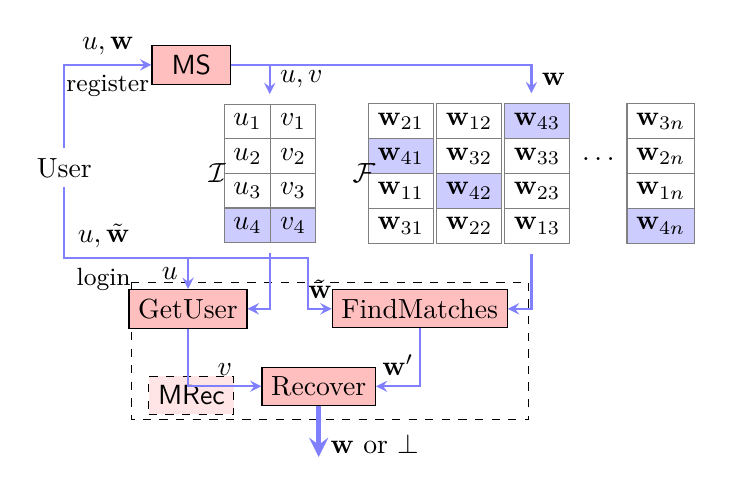
\begin{tikzpicture}[
    >=stealth,
    node distance=2cm,
    database/.style={
      cylinder,
      cylinder uses custom fill,
      cylinder body fill=black!25!white,
      cylinder end fill=black!25!white,
      shape border rotate=90,
      aspect=0.25,
      minimum width=2em,
      minimum height=2em,
      draw
    },
    func/.style={
      rectangle,
      fill=red!25!white,
      minimum width=1cm,
      minimum height=1em,
      draw
    },
    cell/.style={
      rectangle,
      draw=black!50!white
    }
    ]
    \node (user) at (0, 0) {User};
    \node[func, right of=user, right=-1.1em, above=3em] (msketch) {$\MS$}; 
    \draw[below of=msketch, dashed, anchor=west] (.85,0.55) rectangle (5.9,-1.2); 
    \node[func, below of=msketch, anchor=east, below=1.95cm,fill=red!10!white,dashed] (mrecover) {$\MRec$};
    % \node[database, right of=user, anchor=south, above=1em, right=2cm] (db1) {$\dbid$};
    \matrix (db1) [right of=user, anchor=south, below=2pt, right=-0.1cm, 
    matrix of math nodes,
    column sep = -\pgflinewidth,
    row sep=-\pgflinewidth,
    column 1/.style={nodes={cell}}, 
    column 2/.style={nodes={cell}}, 
    anchor=west] {
      \u_1 & \sketchval_1\\
      \u_2 & \sketchval_2\\
      \u_3 & \sketchval_3\\
      |[draw,fill=blue!20]|\u_4 & |[draw,fill=blue!20]|\sketchval_4\\
    };
    \node[left of=db1, anchor=east,right=1.1cm] {$\dbid$};
    \matrix (db2) [right of=db1, left=25pt, matrix of math nodes,
    column sep = 2\pgflinewidth,
    row sep=-\pgflinewidth,
    column 1/.style={nodes={cell}},
    column 2/.style={nodes={cell}}, 
    column 3/.style={nodes={cell}}, 
    column 4/.style={nodes={cell}}, 
    column 5/.style={nodes={cell}}, 
    anchor=west] {
      \mvec_{21} &\mvec_{12} & |[draw,fill=blue!20]|\mvec_{43} &  & \mvec_{3\mlen} \\
      |[draw,fill=blue!20]|\mvec_{41} &\mvec_{32} & \mvec_{33} & |[draw=white]|\ldots & \mvec_{2\mlen} \\
      \mvec_{11} &|[draw,fill=blue!20]|\mvec_{42} & \mvec_{23} &  & \mvec_{1\mlen} \\
      \mvec_{31} &\mvec_{22} & \mvec_{13} & & |[draw,fill=blue!20]|\mvec_{4\mlen} \\
    };
    \node[left of=db2, left=-4pt] {$\dbmsg$};

    % \node[database,right of=db1] (db2) {$\dbmsg$};
    \node[func,below of=db1,anchor=north,above=8pt,left=8pt] (gu) {GetUser};
    \node[func,right of=gu,anchor=east,right=-5pt] (fm) {FindMatches};
    \node[func,below of=db1,anchor=east,below=2em,right=-3pt] (recover) {Recover};

    \draw[->,blue!50,thick] (user.north) |- node[black,near end,above]{$u, \mvec$} node[black,near end,below,font=\small]{register} 
    (msketch.west);
    \draw[->,blue!50,thick] (msketch) -| node[black,near end, left,right]{$u, \sketchval$} (db1);
    \draw[->,blue!50,thick] (msketch) -| node[black,near end, left,right]{$\mvec$} (db2);

    \draw[->,blue!50,thick] (user.south) |- ++(1,-0.9) node[black,near end,above]{$u, \mvectilde$} node[black,near end,below,font=\small]{login}   -| node[black,left,near end]{$u$}
    (gu.north);
    \draw[->,blue!50,thick] (user.south) |- ++(0,-0.9)  -- ++(3.1,0) |- node[black,near end, above]{$\mvectilde$}
    (fm.west);
    \draw[->,blue!50,thick] (db1.south) |- node[black,near end,above]{} (gu.east);
    \draw[->,blue!50,thick] (db2.south) |- node[black,near end,above]{} (fm.east);
    \draw[->,blue!50,thick] (gu.south) |- node[black,near end,above]{$\sketchval$} (recover.west);
    \draw[->,blue!50,thick] (fm.south) |- node[black,near end,above]{$\mvec'$} (recover.east);    
    \draw[->,blue!50,line width=2pt] (recover.south) -- node[black,near end,right]{$\mvec$ or $\bot$} ++(0, -0.65);
  \end{tikzpicture}
  % \rcnote{Rough sketch of the flow of the \biosketch.} 
  \caption{Diagram of multisketch as a part of an authentication service. 
  }
  \label{fig:mainflow}
\end{figure}

%%% Local Variables:
%%% mode: latex
%%% TeX-master: "../main"
%%% End:


You refer to a figure in the following way. In~\figref{fig:mainflow} we show
some thing that is relevant for the Multisketch paper by Chatterjee et
al.~\cite{chatterjee2019multisketches}. Add your bibliography to the
\textsf{bib.bib} file. You can copy the Bibtex format citation from Google
Scholar.

\section{Tools and Methods}
\begin{itemize}
    \item \textbf{Device:} Samsung Galaxy S23 Ultra smartphone, running Android 15, equipped with the Snapdragon 8 Gen 2 Qualcomm SM8550-AB chipset, which supports dual-frequency, multi-constellation GNSS (GPS, Glonass, NavIC, Beidou, Galileo, QZSS). \cite{samsungs23ultra}
    \item \textbf{GNSS data collection:} "GNSSLogger" app, version 3.1.0.4 \cite{gnssLoggerApp} | "GPSTest" app, version 3.10.5 \cite{gpsTestApp} | "Google Earth" app, version 10.79.0.3. \cite{googleEarthApp}
    \item \textbf{Geoid height calculator:} GeographicLib web app. \cite{geoidHeightCalculator}
    \item \textbf{Data analysis:} MATLAB R2024b \cite{matlab} | gps-measurement-tools suite \cite{gpsMeasurementToolsCodebase}, developed by Google, enhanced by the NavSAS research group of Polytechnic of Turin \cite{navSAS} | "Location Based Analysis of Visible GPS Satellites" example notebook from MATLAB Satellite Communications Toolbox. \cite{skyplotsNotebook}
\end{itemize}
Every log contains 5 minutes of uninterrupted data sampled at [45.047208 N, 7.655716 W, 250 m a.s.l.] (Parco Cavalieri di Vittorio Veneto, Turin, Italy) (fig. \ref{fig:map}), isolated approximately 20 meters from nearby obstructions and under fair weather conditions, ensuring minimal multipath interference and optimal
reception. All user-space power-saving options were turned off and the device was put in Airplane mode during logging.
\label{sec:tools}

\section{Open-sky conditions}
\label{sec:opensky}
\subsection{Raw measurements - HW clock de-sync}
% To evaluate the quality and consistency of raw GNSS measurements on Android smartphones, we analyzed data collected from a Samsung Galaxy S23 Ultra in Airplane mode, using: \textbf{GNSSLogger} (developed by Google) and \textbf{GPSTest} (an open-source GNSS diagnostic tool). 

% Data collection was carried out in Parco Cavalieri di Vittorio Veneto, located in Torino, Italy, under clear weather conditions. The test device was placed in an open-sky environment, isolated approximately 20 meters from nearby obstructions (fig. \ref{fig:map}), ensuring minimal multipath interference and optimal reception of the GNSS signal. 
% To ensure maximum measurement continuity and stability, all adaptive battery saving features of the operating system were disabled, including background activity restrictions and battery optimization settings for GNSSLogger. This was done to prevent throttling or suspension of GNSS-related processes during data logging.

During our first experiment, which we conducted under all conditions specified in \ref{sec:tools}, we observed hardware clock discontinuities that directly affected the reliability of pseudorange computations.


\begin{figure}[H]
        \centering
        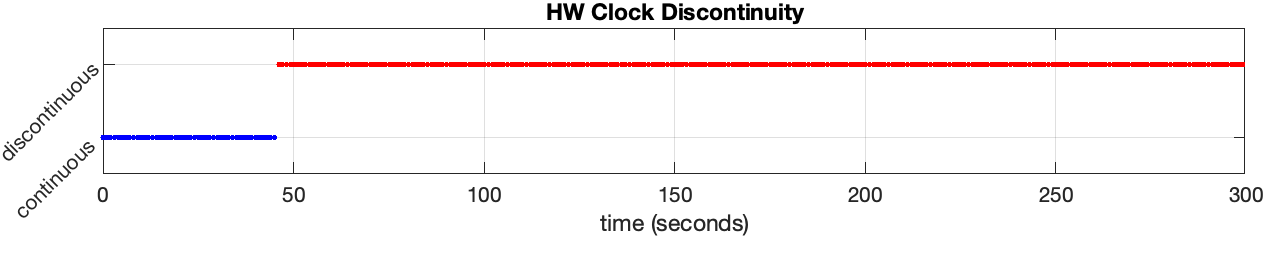
\includegraphics[width=0.85\linewidth]{images/discontinuity_gnss_log.png}
        \caption{Status of GNSS hardware clock over time with just GNSSLogger}
        \label{fig:GNSSLogger-discontinuity}
\end{figure}

Although no power-saving modes of any kind were active in the mobile device, HW clock discontinuities, indicated by a transition from blue (continuous) to red (discontinuous), were detected at approximately 46 seconds into the logging session and persisted for the duration of the test (fig. \ref{fig:GNSSLogger-discontinuity}).
This discontinuity indicates that the device’s internal clock experienced a sudden and irregular change in its progression. Instead of increasing smoothly over time, the clock may have jumped forward, backward, or altered its rate. This issue is not caused by a loss of synchronization with GNSS time, which is always managed through a clock bias, but rather by a sudden instability in the internal device clock that breaks the assumption of consistent bias over time. As a result, time-dependent computations, such as speed estimation or pseudorange rate, become unreliable from the point of discontinuity onward.

% \colorbox{red}{https://sites.google.com/view/gnsstutorial}
\begin{figure}[H]
    \centering
    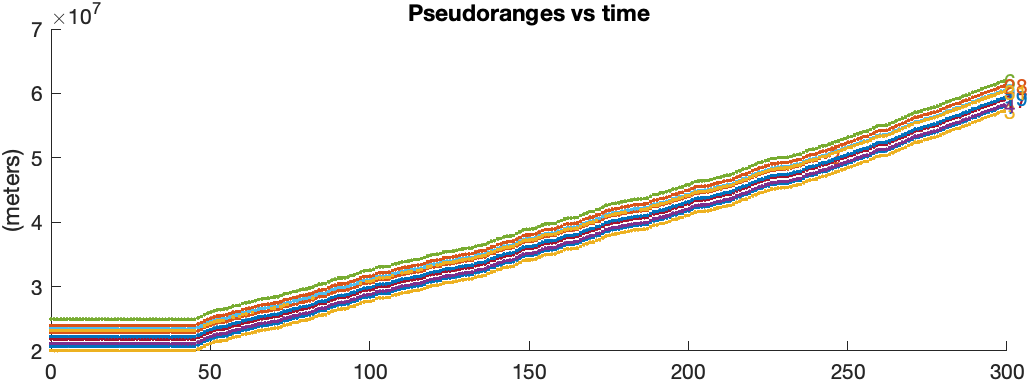
\includegraphics[width=0.75\linewidth]{images/disontinuity_pseudorange_vs_time.png}
    \caption{Pseudoranges vs. time under HW clock discontinuity}
    \label{fig:disontinuity_pseudorange_vs_time}
\end{figure}

As shown in Figure \ref{fig:disontinuity_pseudorange_vs_time}, after the clock discontinuity occurs, all pseudorange values begin to increase steadily and appear very similar across all satellites. This unusual pattern is caused by an incorrect handling of the clock bias during the computation of the GNSS receive time (\textit{tRxNanos}).

In the script, \textit{tRxNanos} is calculated using the expression:
\begin{equation*}
    \label{eq:tRxNanos}
    \text{tRxNanos} = \text{TimeNanos} - \text{FullBiasNanos}(1) - \text{weekNumberNanos}
\end{equation*}
where \textit{TimeNanos} is the internal time of the device at the moment of signal reception, \textit{FullBiasNanos} is the correction term that accounts for the difference between the device’s clock and true GNSS time, and \textit{weekNumberNanos} adjusts for GPS week rollovers.

However, the script applies a constant \textit{FullBiasNanos} value across the entire dataset, using the one extracted from the first epoch (\textit{FullBiasNanos(1)}). In reality, the clock bias is not constant: it can drift over time or change abruptly in the presence of a clock discontinuity. When this happens, \textit{TimeNanos} may suddenly jump, but since the bias is not updated accordingly, it no longer compensates correctly. This causes \textit{tRxNanos} to become inaccurate from that point on, introducing a common shift in the receive time for all satellites.
This has a significant effect on the pseudorange calculation, which is defined as:
\begin{equation*}
    \text{pseudorange} = (tRx - tTx)c
\end{equation*}
where \textit{tRx} is the receiver time computed as \ref{eq:tRxNanos}, \textit{tTx} is the transmission time from the satellite and \textit{c} is the speed of light.
When the signals from the satellites arrive at the same time, \textit{tRx} will be identical for all of them. In this case, the differences in the pseudoranges are determined solely by the \textit{tTx}, the timestamp of each satellite’s signal transmission. However, even a small error in \textit{tRx}, in the order of microseconds (as showed in \ref{fig:discontinuity_bias_clock}), can result in a large pseudorange error because it is multiplied by the speed of light. As a result, the pseudoranges may appear almost identical in the graph due to this large error, which grows over time.

Despite these errors in PR computation, the estimated positions remain approximately correct. This is because the weighted least squares solution simultaneously estimates not only the receiver’s position and velocity but also the clock bias as an unknown parameter. As a result, even if the initial bias used in the pseudorange computation is outdated or incorrect, the solver adjusts the bias dynamically during the estimation process. However, since the initial PR inputs are distorted by the uncorrected bias, the system starts from less precise measurements, which can slightly degrade the accuracy of the estimated position and velocity (fig. \ref{fig:discontinuity_map_computed_position_vs_true_postion}).

\begin{figure}[H]
    \centering
    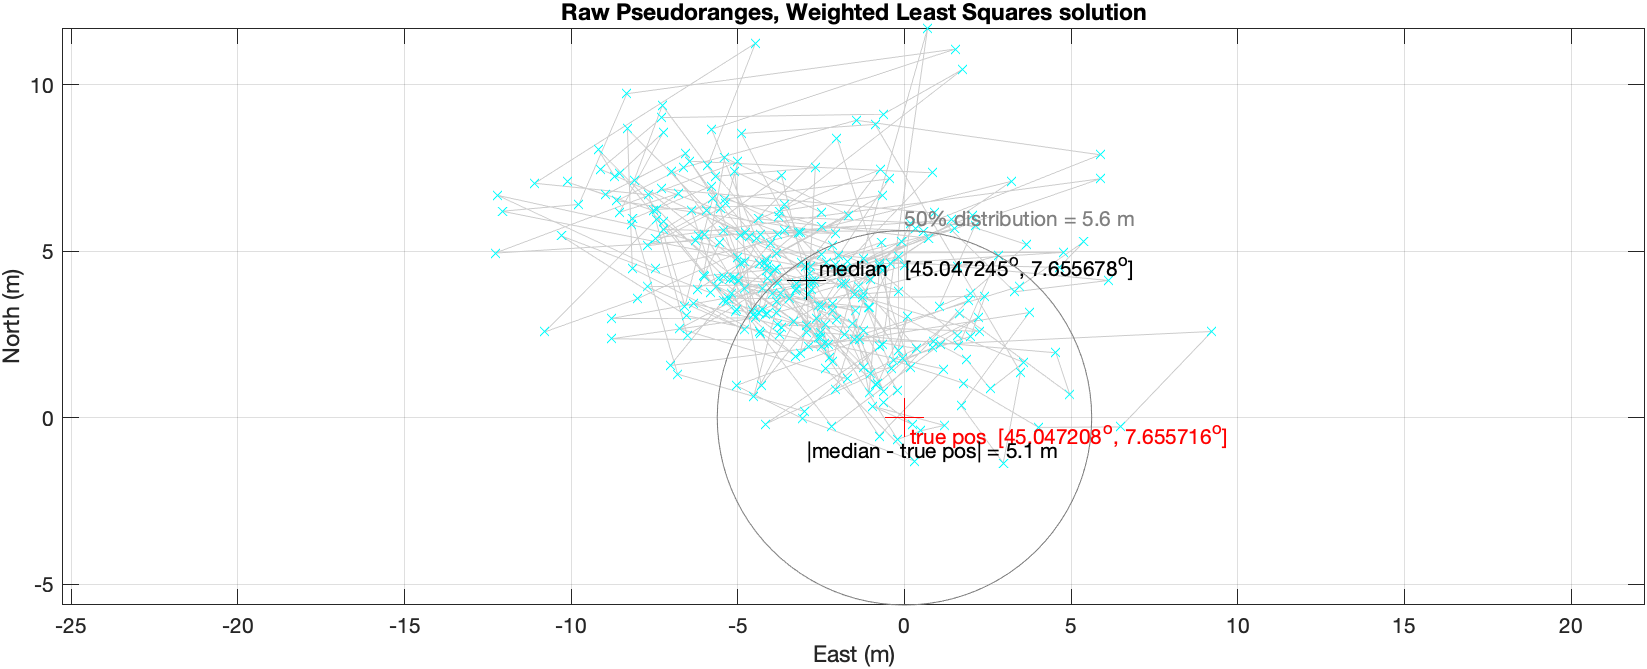
\includegraphics[width=0.85\linewidth]{images/discontinuity_map_computed_position_vs_true_postion.png}
    \caption{Computed position with discontinuity clock vs true position}
    \label{fig:discontinuity_map_computed_position_vs_true_postion}
\end{figure}

\subsubsection{Solving the HW clock discontinuity}
 
While the WLS algorithm partially compensates for bias errors, a better solution was found by directly preventing the discontinuities from occurring.
In particular, launching the GPSTest \cite{gpsTestApp} app in parallel with GNSSLogger during data collection sessions eliminated HW clock discontinuities (fig. \ref{fig:GNSSLogger-continuity}). 

% As shown in fig. \ref{fig:GNSSLogger-continuity}, the hardware clock remained continuous for the full duration of the experiment.
This behavior suggests that the root cause is not related to external environmental factors, but rather stems from the internal management of GNSS resources on the Android platform, like foreground priority and wake locks, leading to clock resets or timing irregularities.
By forcing continuous GNSS activity through GPSTest, this behavior is suppressed entirely, and the hardware clock remains stable throughout the session.

In order to obtain better results, without discontinuity, all subsequent surveys were carried out using the two applications, GNSSLogger and GPSTest, run in parallel.


\subsection{Raw measurements - no HW clock de-sync}
Having solved the HW clock de-synchronization issue, the logging produced the best samples we had, which we will use as a baseline to analyze worse scenarios. Correlating the logs with the visibility skyplot produced by the MATLAB notebook \cite{skyplotsNotebook} (fig. \ref{fig:skyplot_punto_3}), we can see how the phone's receiver has been continuously able to receive signals from all visible satellites, except for satellites 20, 26 and 30, which were possibly out of sight because of their low elevation angle of less than 10 degrees above the horizon. In addition, HDOP has been stable at a value of 0.8 (fig. \ref{fig:hdop_punto_3}), which indicates very good geometrical conditions.

The C/N0 plot (fig. \ref{fig:CN0_punto_3}) shows how the intensities of signals from visible satellites have no immediate correlation with the elevation angle; in particular, we see how satellites closer to our Zenith and closer in terms of straight-line distance, as shown by the pseudoranges (fig. \ref{fig:pseudoranges_opensky}), are not among the strongest signals we received. Finally, some signals were surely more stable in their intensity than others; examples of this behavior are satellite 4 (very stable at more than 50 dB-Hz) and satellite 7 (oscillating in a range between 30 and 45 dB-Hz).

\begin{figure}[H]
    \centering
    \begin{minipage}[b]{0.40\linewidth}
        \centering
        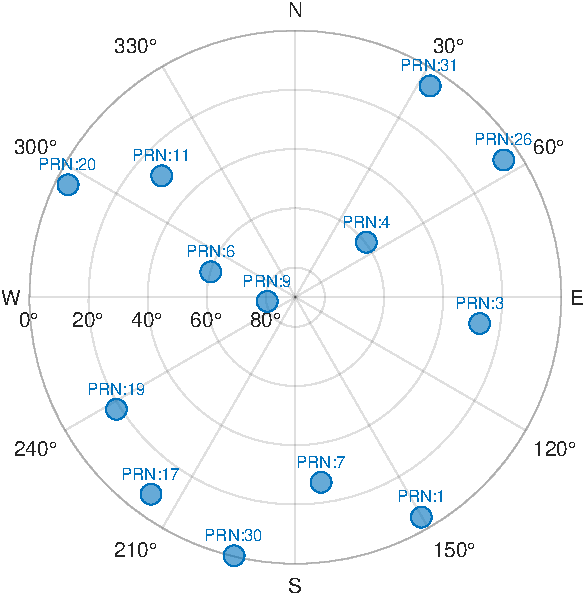
\includegraphics[width=\linewidth]{images/skyplot_punto_3.pdf}
        \caption{Skyplot of visible satellites at 20:16:32 UTC+2}
        \label{fig:skyplot_punto_3}
    \end{minipage}
    \hfill
    \begin{minipage}[b]{0.56\linewidth}
        \centering
        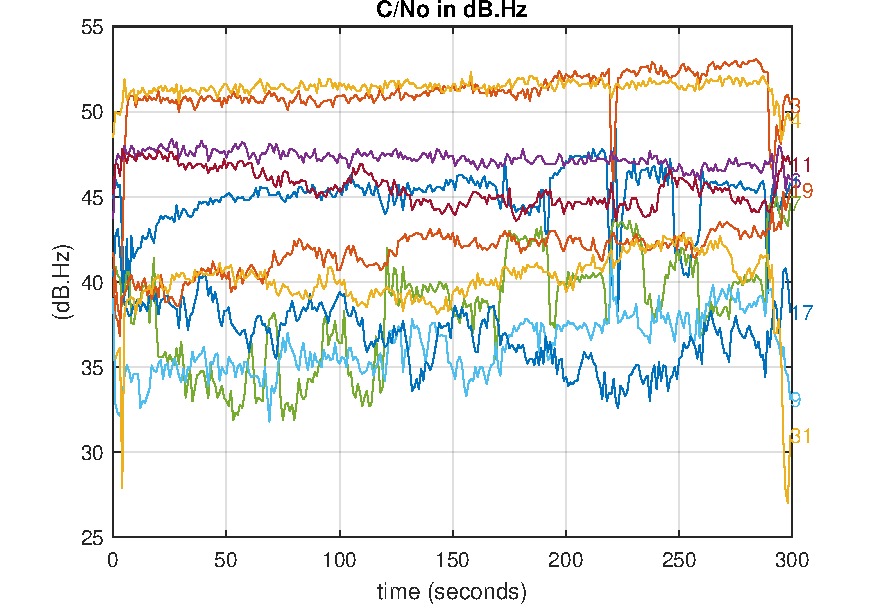
\includegraphics[width=\linewidth]{images/CN0_punto_3.pdf}
        \caption{Carrier to noise density ratio, dB-Hz}
        \label{fig:CN0_punto_3}
    \end{minipage}
\end{figure}

\subsection{Position, Velocity and Time}
The open-sky conditions are also reflected in the quality of the results obtained in terms of position, velocity and time estimation. We obtained very stable results; the 50\% computed positions were within a circle of radius of 1 m (fig. \ref{fig:pos_punto_3_precision}), with an error of 5.4 meters between the median and the real position (on the horizontal plane) (fig. \ref{fig:pos_punto_3}). 

However, comparing the estimated altitude with the actual one (obtained via Google Earth), we observed a significant discrepancy, not only due to the precision of the GNSS system, but also to the difference in models used to represent the shape of the Earth \cite{esriGeoidArticle} \cite{eosElevation2025}. In particular, Google Earth uses the EGM96 geoidal model for the planet \citep{googleEarthModel} \citep{googleEarthModel2}, and therefore refers to an orthometric height, while the script we used relies on the WGS84 ellipsoid model, and outputs an ellipsoid height. The geoid height for the specific location is easily retrieved by using online tools \cite{geoidHeightCalculator}. 

% ellipsoid is lower than geoid, like in our case. If changing this, change it to something similar.
\begin{figure}[H]
    \centering
    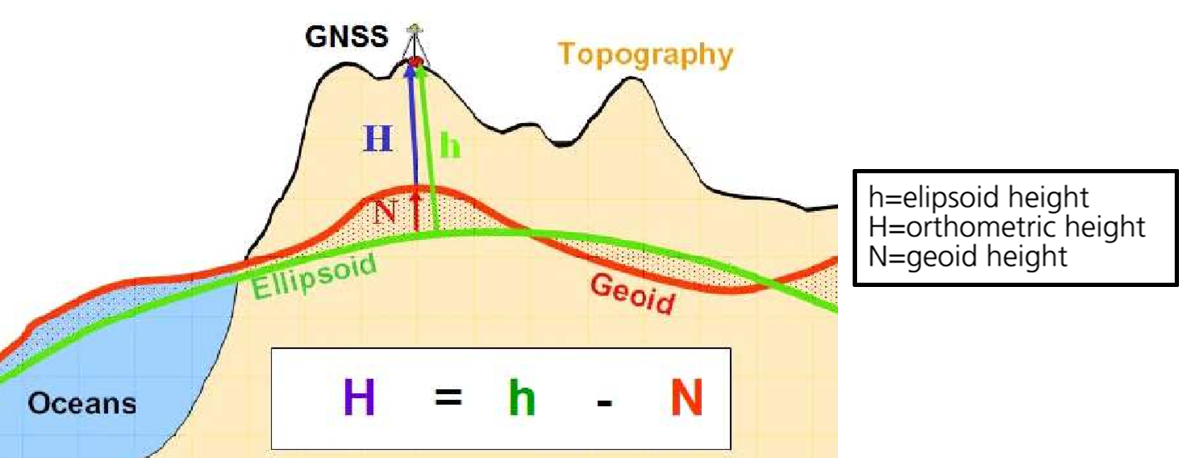
\includegraphics[width=0.50
    \linewidth]{images/geoidellipsoid_legenda.png}
    \caption{Orthometric and ellipsoid height, taken from \cite{kaminskis2008quasigeoid}.}
    \label{fig:h=H+N}
\end{figure}

In our case, the median altitude  reported by the MATLAB tool ($h$) was 321 m, the one obtained from Google Earth ($H$) was 250 m and the geoid height in our location ($N$) is 48 m, so the error in the altitude estimation is $h - (H + N) = (321 - 250 - 48)\ \SI{}{\meter}= \SI{23}{\meter}$, which aligns with our expectations about the vertical accuracy \cite{Enge2010-uj}.



% This leads to an altitude difference that is measured by subtracting the geoid height from the ellipsoid height - equivalently, it's the difference between orthometric height and geoid height at the location being evaluated (which is easily retrieved by using online tools \cite{geoidHeightCalculator}) \cite{esriGeoidArticle}. 



\section{Cyber-spoofing simulation}
\label{sec:spoofing}
\subsection{Altering pseudoranges}
\label{subsec:altering_pseudoranges}
As a first experiment with our cyber-spoofing emulation, we operated on the logs collected in \ref{sec:opensky}. We chose to spoof our location 1 Km away from the real one, at the same altitude, of coordinates [45.0487414 N, 7.6682227 W]. The spoofing process computes, for each satellite in sight, the difference in the pseudorange that would be observed between the true location and the spoofed location; it then derives satellite-dependent time delays, which it adds to each log entry from that satellite.
In our setting, spoofing starts at $t = 150$ s, exactly in the middle of the logs collection period. 
\subsubsection{Effects on raw measurements}
\label{subsec:effects_raw_meas}
We were expecting both a sudden jump in the pseudoranges and a visible spike in the middle of the PRRs (when computed at runtime as a ratio of deltas, rather than being parsed from the logs). However, we observed that plotting PR amplitudes over time is not enough to visually notice the introduced difference while visualizing the behavior of more curves at once. 

Instead, considering only how the PR changes from their initial values, the jump is more evident. In fact, given that the receiver was standing still while collecting GNSS data, the plotted curves will be straight lines with a fairly stable slope while spoofing is not active, due to the natural movement of the SATs. By plotting only the slopes of those curves over time, which are a fair approximation of the PRRs, we see how the SAT-specific deltas added to the pseudoranges translated into a visible spike in each of the curves at $t = 150$ s (fig. \ref{fig:spoofing_no_delay_prrs}). This pulse-shaped alterations are far more readable to the eye and at the same time suggest that the absolute modifications over the pseudoranges were rather small. 

\begin{figure}[H]
    \centering
    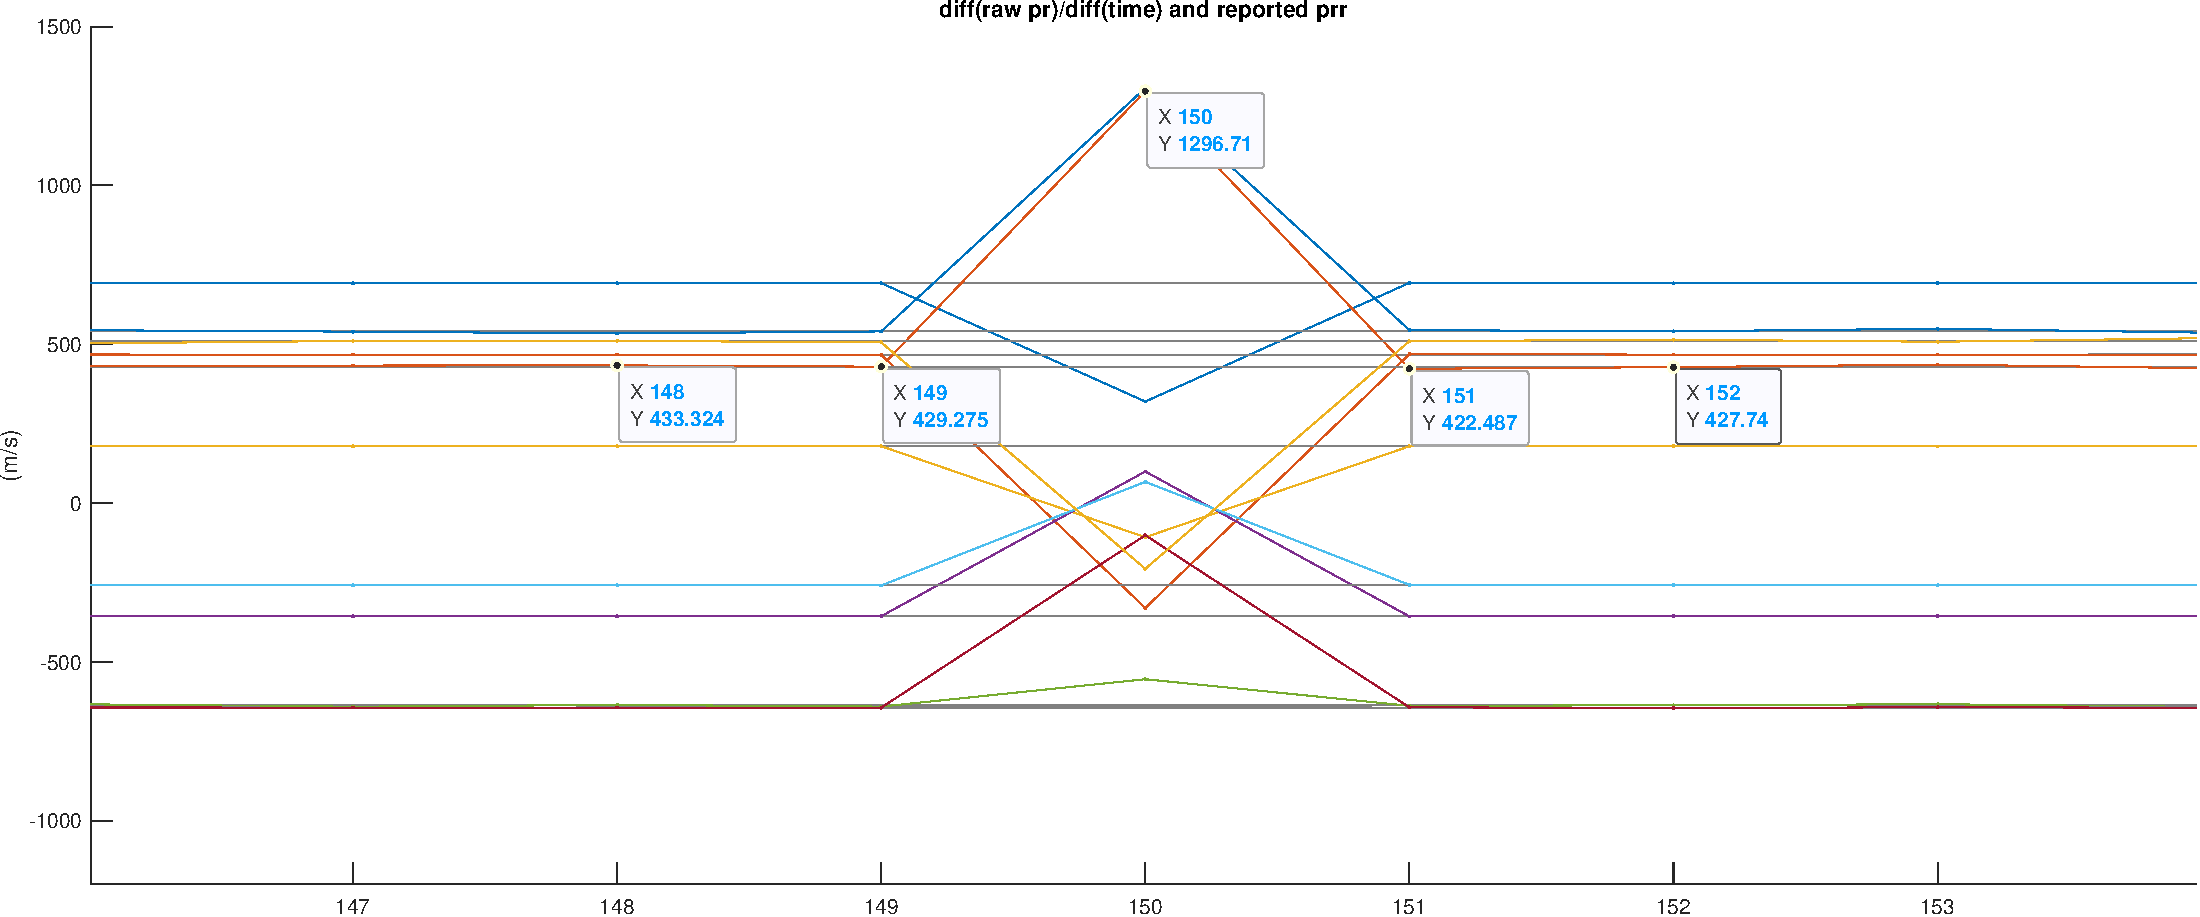
\includegraphics[width=0.75
    \linewidth]{images/1KM_spoofing_prr_of_sat_19}
    \caption{Pseudorange rates computed as ratios of deltas, or slopes of PR change from initial value over time. Tooltips show data about satellite 19.}
    \label{fig:spoofing_no_delay_prrs}
\end{figure}

Let's focus on SAT 19. Its pseudorange was about $2.25\cdot 10^7$ m during the whole logs collecting operation (fig. \ref{fig:pseudoranges_opensky}), and it was one among the most affected satellites by our spoofing. Its PR was also naturally changing due to the satellite moving, with a slope of about 430 m/s; the spoofing introduced a spike of about 1300 m/s at $t = 150$ s.

We can conclude that to trick the positioning algorithm into a location that was 1 Km away from the real one, each pseudorange has been altered by at most 0.00004\% of the value they had a second before the spoofing started. This really enhances our perspective on how the GNSS receivers rely on the smallest variations in the signal reception times to produce their outputs.

\subsubsection{Effects on PVT solution}
\label{sec:fratm}
While the most obvious effect of the spoofing simulation is the sudden change in positioning (fig. \ref{fig:pos_spoofed_no_delay}), the effects on the velocity states surely deserve attention. In fact, it's clear how velocities do not correspond to the ratios between the point-to-point distance and the time between two epochs, otherwise the velocity plots would present a visible spike in the middle, just like the plot of pseudoranges rates (fig. \ref{fig:spoofing_no_delay_prrs}).

Instead, velocities are being computed by exploiting the Doppler shift phenomenon \cite{psuDopplerShift2025}, because of which the signals from SATs are perceived by the receiver at slightly different frequencies, depending on the relative motion between the SAT and the receiver. Our receiver catched these subtle frequency shifts and autonomously derived PRRs (which here are to be interpreted as relative velocities between the receiver and the specific SAT) that we can find in the log entries (fields \textit{PseudorangeRateMetersPerSecond} and \textit{PseudorangeRateUncertaintyMetersPerSecond}). 

The MATLAB tool \cite{gpsMeasurementToolsCodebase} we used for the analysis has exploited those values, which our spoofing algorithm did not modify in any way, to estimate the velocity of the receiver; in particular, the WLS solver had to compensate the fact that in our new position we still had the previous relative velocity with respect to each of the SATs, which it did by tweaking the velocity estimates in both amplitude, direction and variance. This behavior justifies what we see in fig. \ref{fig:spoofing_velocities_no_delay}.

\begin{figure}[H]
    \centering
    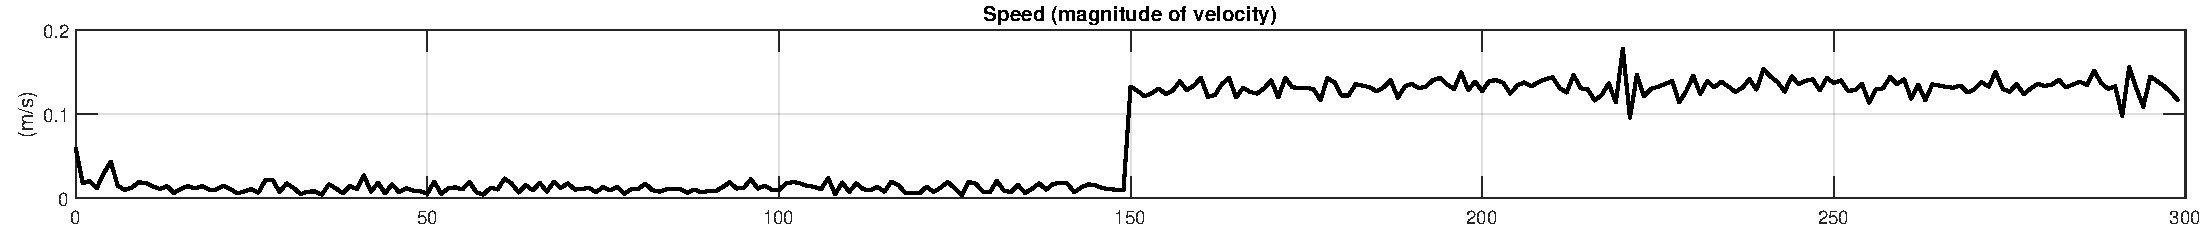
\includegraphics[width=1.00
    \linewidth]{images/spoofing_velocities_no_delay.pdf}
    \caption{Velocity states over time after spoofing}
    \label{fig:spoofing_velocities_no_delay}
\end{figure}

\subsection{Spoofing detection}
During the various tests we conducted, we made an attempt to identify methodologies for detecting ongoing cyber-spoofing activities.
% It should be noted that the following analysis is not highly precise, as the spoofing technique employed by the MATLAB tool \cite{gpsMeasurementToolsCodebase} differs from those typically used in real-world scenarios. Specifically, it operates by "falsifying" already recorded GNSS logs so that the resulting calculations return a spoofed position. In this context, certain warning signs can be identified. 
\subsubsection{Spikes in the runtime-computed pseudorange rates} 
\label{sec:boh}
From the analysis of the pseudorange rates graph, not only we see how the computed PRRs differ from the logged ones (the gray curves), but we also observe distinctive spikes, which occur when the PR value changes abruptly from one epoch to the next (fig. \ref{fig:spoofing_no_delay_prrs}).
When the spoofed location is far enough, the magnitude of the spike stands out clearly from the background noise, facilitating detection. 
% \colorbox{red}{TODO: inserire grafico picco derivata in relazione al rumore di fondo}

Moreover, since our spoofing technique involves adding deltas to all visible satellites starting from a selected timestamp, the spikes present themselves simultaneously, which allows to distinguish the spoofing event even in the case of spikes of lower amplitude. 
% \colorbox{red}{TODO: inserire grafico picco derivata visibile contemporaneamente su più satelliti}. 
\subsubsection{Inconsistent velocity states}
As previously mentioned, the spoofing emulation introduces anomalies in the velocities (\ref{sec:fratm}).
% To explain this more precisely: GNSS receivers are capable of estimating the velocity of the user not only through changes in position over time, but also through analysis of the Doppler shift — the variation in the frequency of the signal received from each satellite.
% If a satellite moves toward the receiver, the signal’s frequency appears slightly higher than its nominal value; conversely, if it moves away, the frequency appears lower.
% By measuring these frequency shifts for multiple satellites, the receiver can reconstruct the complete 3D velocity vector of the device with high accuracy. This Doppler-based velocity is independent from the pseudorange-based position calculation.

% However, when spoofing is introduced using the Google tool, this mechanism breaks. The spoofing affects only the pseudorange data (i.e., the perceived position), while the frequencies and Doppler shifts remain unchanged and still reflect the true physical position of the receiver.
% This inconsistency leads to the detection of sudden and unrealistic velocity changes. 

For instance, the sudden increase in speed that the WLS solver introduces when the spoofing starts may not be wide enough to justify the position shift. In our example, the spoofed position was 1 Km away from the real one, but velocity peaked at less than 0.2 m/s, instead of showing a spike reaching 1 Km/s in $t = 150$ s (which would have have been unrealistic nonetheless, in terms of acceleration) (fig. \ref{fig:spoofing_velocities_no_delay}).

A more complex cyber-spoofing strategy, which would also alter the pseudorange rates, would probably cancel this behavior, but is also likely to be detected by searching for sudden changes in the PRRs themselves, or by correlating such values to data taken from other sensors the system is equipped with, such as accelerometers.
\subsection{Adding time delay}
\label{subsec:time_delay}

Starting the spoofing attack at $t = 150$ s and using the previously spoofed position, we set the variable \textit{spoof.delay} = 0.003, meaning a 3 ms delay. Essentially, the script now not only will modify the signal reception times by adding SAT-dependent delays, but also simulate that they all were received 3 ms later than they actually were.
The change in delay creates a scenario very similar to a meaconing attack. In fact, the only difference here is that we are applying an additional common delay to all the satellite signals, that will be incorporated into the receiver's clock bias. This bias will be estimated and accounted for during the calculation by the WLS solver. The resulting change in the bias due to this delay is evident in figure \ref{fig:spoofing_clock_bias_with_delay}.
\begin{figure}[H]
    \centering
    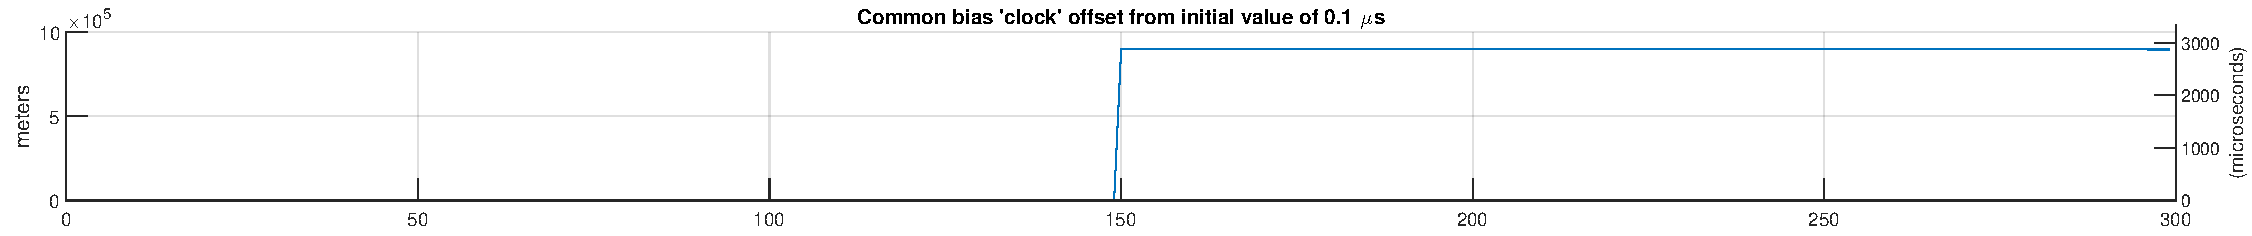
\includegraphics[width=1.00
    \linewidth]{images/clock_bias_with_delay.pdf}
    \caption{Common user clock bias after spoofing with additional delay}
    \label{fig:spoofing_clock_bias_with_delay}
\end{figure}
Since this delay change only affects the clock bias, the position will still be calculated correctly. However, unlike the simple spoofing attack, where a very small change in pseudoranges could falsify the position by 1 km, we now observe a larger shift in the pseudoranges, which take on much larger values. This behavior, which we discussed in the first HW clock discontinuity scenario, is due to the growing clock bias, now caused by the delay, which wasn't properly corrected in the graph (fig. \ref{fig:spoofing_pseudoranges_with_delay}).
\begin{figure}[H]
    \centering
    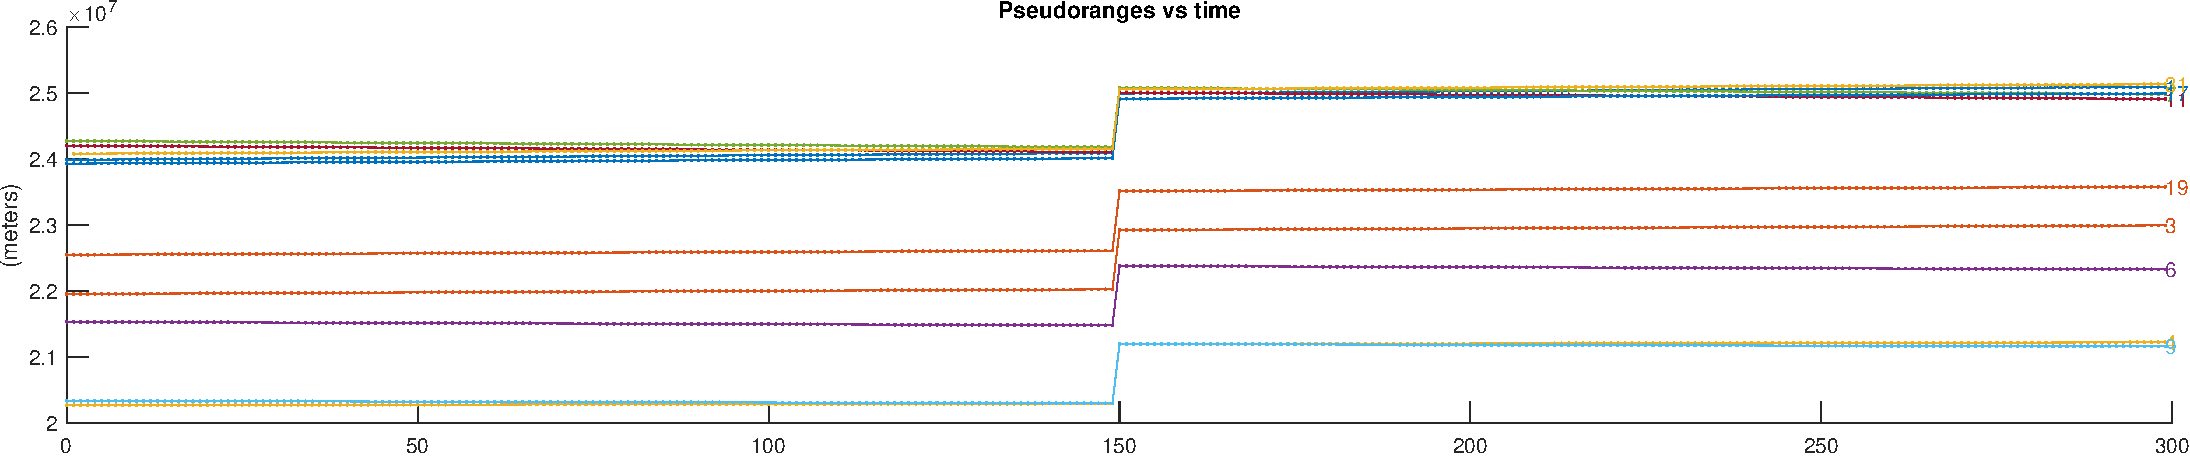
\includegraphics[width=1.00
    \linewidth]{images/spoofing_prs_change_due_to_delay.pdf}
    \caption{Pseudoranges vs. time, after spoofing with  additional delay}
    \label{fig:spoofing_pseudoranges_with_delay}
\end{figure}
\subsection{Interference scenario}
\label{interference}
\subsubsection{Can subdermal GPS microchips enable human tracking?}
The feasibility of receiving GNSS signals through human skin is severely limited due to the signal's extremely weak power and the radio-frequency (RF) attenuation properties, especially in the L-band, of biological tissue. 

GNSS signals are very weak and require a line-of-sight to satellites. Human tissue, with its high water and organic content, strongly attenuates these signals such that subdermal reception is extremely unlikely without an external antenna.

\subsubsection{Using minced pork to simulate human tissues for GNSS signal attenuation}
We employed minced pork as a biological analog to human tissues to investigate the attenuation of GNSS signals in subdermal environments. Porcine meat is widely recognized in biomedical research as a suitable surrogate for human tissues due to its comparable physiological and dielectric characteristics \cite{ranamukhaarachchi2016micromechanical}. In addition, it offers a homogeneous medium that facilitates consistent and reproducible measurements. However, while it simplifies experimental conditions, this model lacks the stratified structure of natural skin, which may influence the attenuation characteristics compared to intact tissues.
% By utilizing minced pork, we aim to establish a baseline understanding of how biological tissues can affect the reception of GNSS signals by subdermally implanted devices. This approach allows for controlled experimentation while acknowledging the limitations inherent in the model.

\subsubsection{Scenario analysis}
For this experiment, we replicated the same conditions previously described in \ref{sec:opensky}, maintaining a continuous clock signal without discontinuities. The measurements were repeated the following day at the same time (20:16:32 UTC+2), this time surrounding the device \cite{samsungs23ultra} with a 2.5 cm thick layer of minced pork to simulate subdermal tissue.

To evaluate the effect of biological interference on GNSS signal quality, we compared the Horizontal Dilution of Precision (HDOP) and the number of tracked satellites across two scenarios. In the interference scenario (\ref{fig:carne_hdop}), HDOP values fluctuate noticeably, ranging approximately from 0.9 to 1.4, and the number of SATs varies frequently between 6 and 9. These fluctuations indicate unstable satellite geometry and occasional signal degradation, likely due to the RF attenuation properties of the biological tissue. The increased HDOP and reduced satellite availability correlate with potential deterioration in positional accuracy, consistent with expected GNSS performance under obstructed conditions.
In contrast, in open-sky conditions, the GNSS receiver can maintain high positioning accuracy with minimal dilution effects, as already discussed in (\ref{sec:opensky}).


\begin{figure}[H]
    \centering
    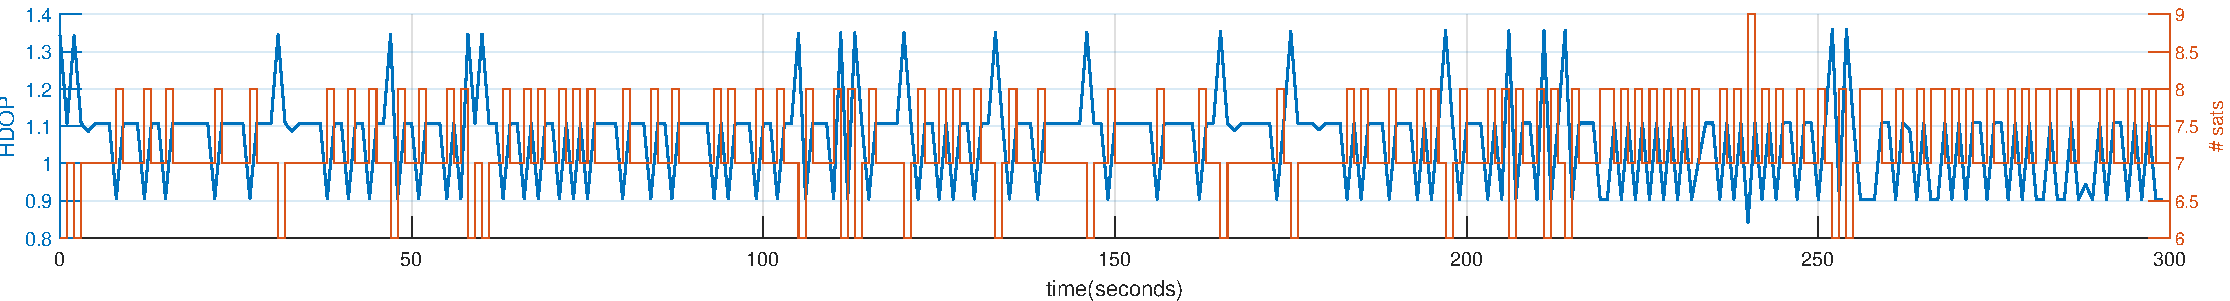
\includegraphics[width=1.00
    \linewidth]{images/carne_hdop_carne.pdf}
    \caption{HDOP and SATs number in the interference scenario}
    \label{fig:carne_hdop}
\end{figure}

\begin{figure}[H]
    \centering
    \begin{minipage}[b]{0.48\linewidth}
        \centering
        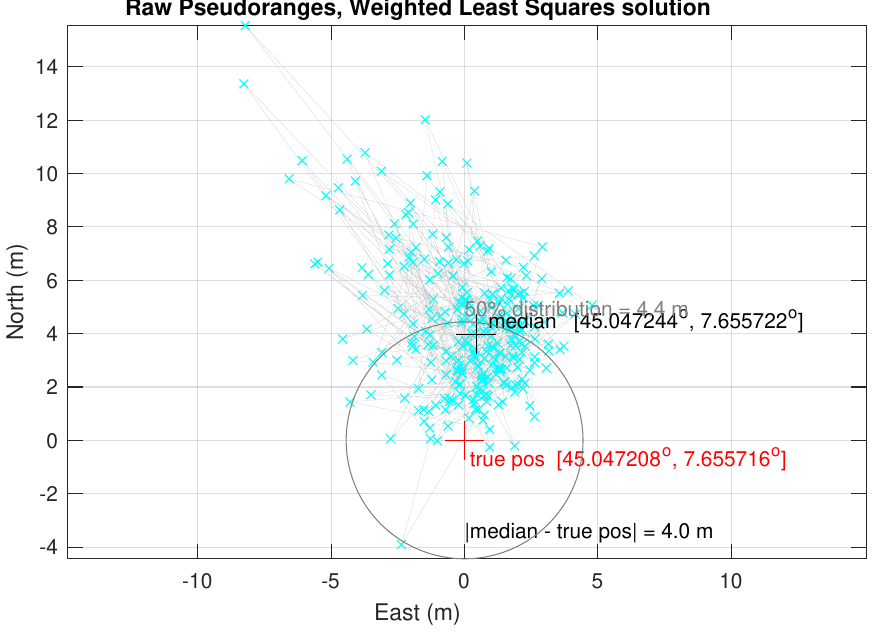
\includegraphics[width=\linewidth]{images/carne_pos.png}
        
        \caption{Positioning in the interference scenario}
        \label{fig:carne_pos}
    \end{minipage}
    \hfill
    \begin{minipage}[b]{0.48\linewidth}
        \centering
        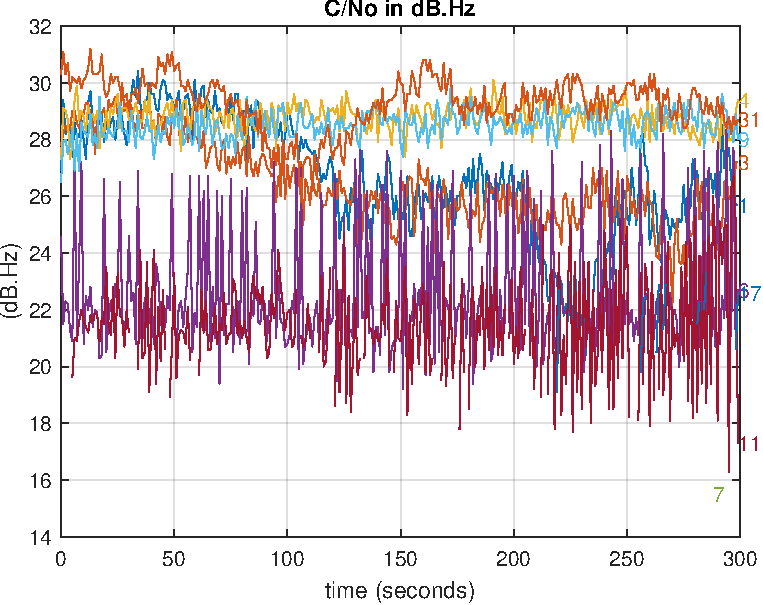
\includegraphics[width=\linewidth]{images/carne_CN0_carne.pdf}
        \caption{C/N0, dB-Hz in the interference scenario}
        \label{fig:CN0_carne}
    \end{minipage}
\end{figure}

Figures \ref{fig:CN0_punto_3} and \ref{fig:CN0_carne} show the Carrier-to-Noise Density Ratio (\(C/N_0\)) measurements under the two conditions, a key indicator of GNSS signal strength and quality, with higher values correlating to better measurement reliability and accuracy. In the interference scenario, most satellite signals exhibit significant attenuation, with \(C/N_0\) values ranging predominantly between 20–30 dB-Hz. The lower and more fluctuating values suggest substantial signal degradation caused by the dielectric absorption and scattering effects of biological tissue. In contrast, in the non-interference scenario, \(C/N_0\) values are consistently higher and less variable, mostly within the 35–50 dB-Hz range, indicating robust and stable signal reception. 

The observed differences between the two conditions provide clear experimental evidence that biological tissue attenuates GNSS signals, reducing the number and the geometry of usable satellites and potentially compromising positioning accuracy. 
% These findings underscore the practical limitations of subdermal GNSS implantation without an external antenna or signal relay mechanism.

In Figure \ref{fig:carne_pos}, we observe an interesting outcome: although measurements are generally more precise in the open-sky scenario (fig. \ref{fig:pos_punto_3_precision}), the results in the interference setting show a median only 4 m away from the real position. This may be due to a sort of filtering effect of the biological material, which limits the number of usable satellites to the ones that had a stronger and more stable signal.

However, this apparent gain in accuracy does not correlate to a better precision (fig. \ref{fig:accPos}), as the various position states appear more scattered (see also fig. \ref{fig:carne_pos_precision}), suggesting that biological tissue introduced biases due to signal weakening and poor satellite geometry (HDOP). Therefore, in applications requiring both high accuracy and reliability, biological interference must be considered a non-negligible source of error, reinforcing the impracticality of using unassisted subdermal GNSS devices for precise human tracking.

\section{Conclusion}
\label{sec:conclusion}

% The analysis of the different scenarios clearly shows that wired network transmission maintains a high level of stability. The simplicity of the setup and the use of Ethernet cables allow for accurate theoretical estimations of goodput, as the variables involved are limited and controllable. At the same time, it is clear how this significantly changes when moving to wireless communication. The wide range of technologies and protocols available in 2025 makes it challenging to obtain precise theoretical estimates of goodput, and even after conducting additional analyses, computeing accurate predictions remains complex.  
% Finally, we observed how highly variable environments like saline water make empirical evaluations the only reliable approach.

% In conclusion, this study highlights the importance of considering transmission environment characteristics and device specifications to obtain realistic goodput estimations, especially for wireless and unconventional communication scenarios.

Despite our computations being somewhat approximative, we can still extract valuable insights.
Wired networks offer stable transmission, allowing accurate goodput estimations due to controlled variables. In contrast, wireless communication introduces complexity, making precise theoretical predictions challenging, because of the wide range of technologies of 2025. Finally, empirical evaluation remains essential, particularly in highly variable environments like saline water. 




\onecolumn
\bibliographystyle{ACM-Reference-Format}
\bibliography{bib}
% % --- Appendix ---%
\appendix
\onecolumn
\section{Additional plots}
\label{sec:additional_plots}

\begin{figure}[H]
    \centering
    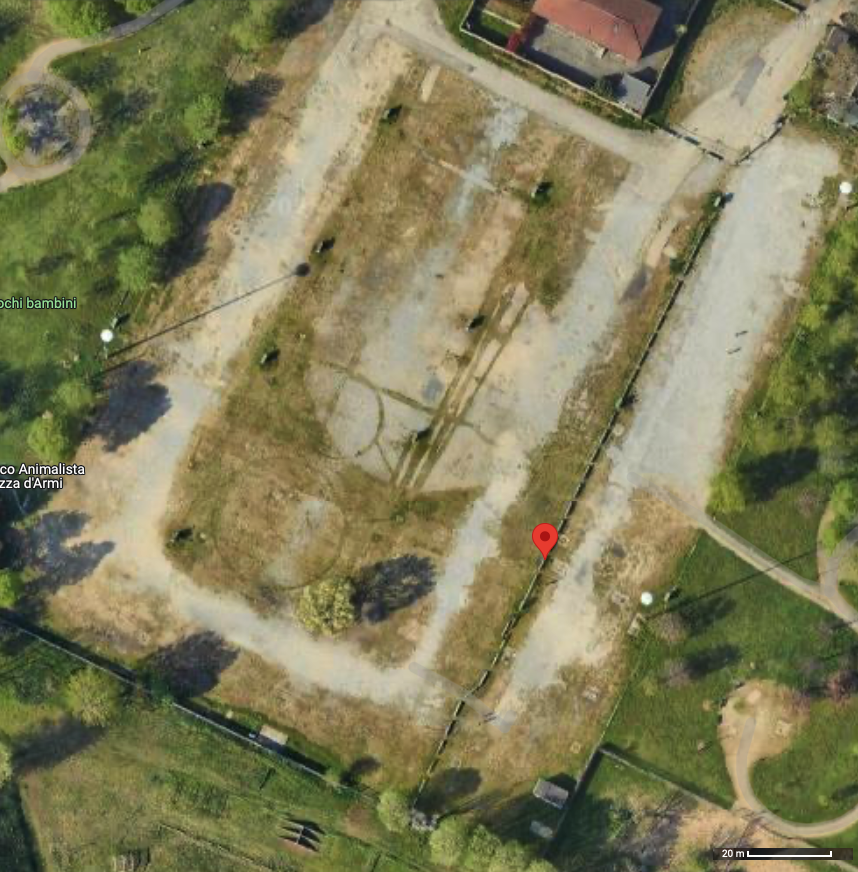
\includegraphics[width=0.5\linewidth]{images/map_place.png}
    \caption{Place where all surveys were carried out.}
    \label{fig:map}
\end{figure}

% \begin{figure}[H]
%     \centering
%     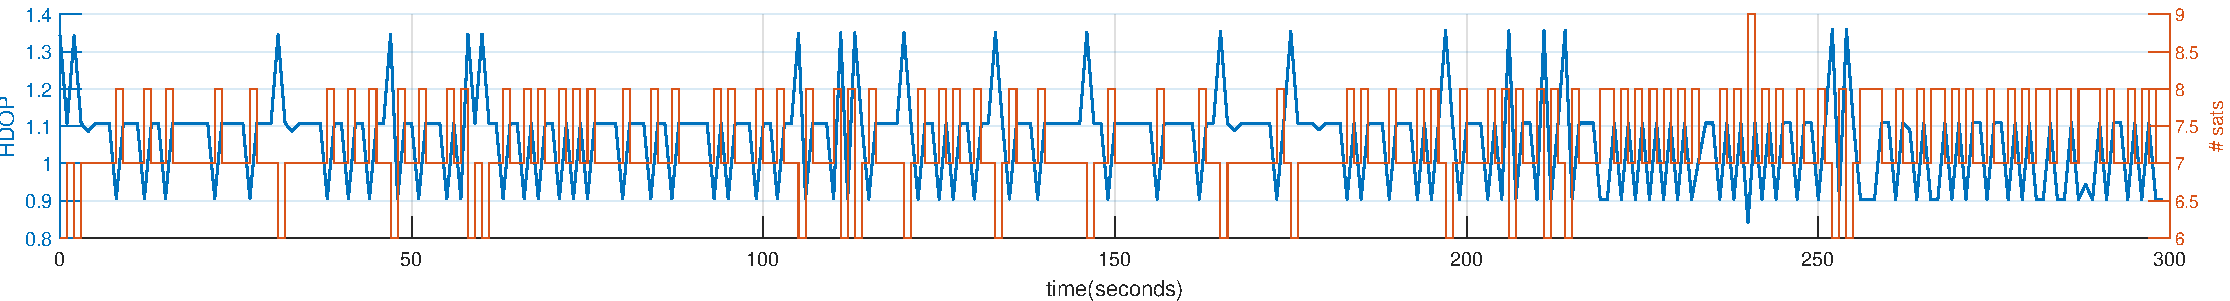
\includegraphics[width=1.00
%     \linewidth]{images/carne_hdop_carne.pdf}
%     \caption{HDOP and SATs number in the interference scenario}
%     \label{fig:carne_hdop}
% \end{figure}

\begin{figure}[H]
    \centering
    \begin{minipage}[b]{0.48\linewidth}
        \centering
        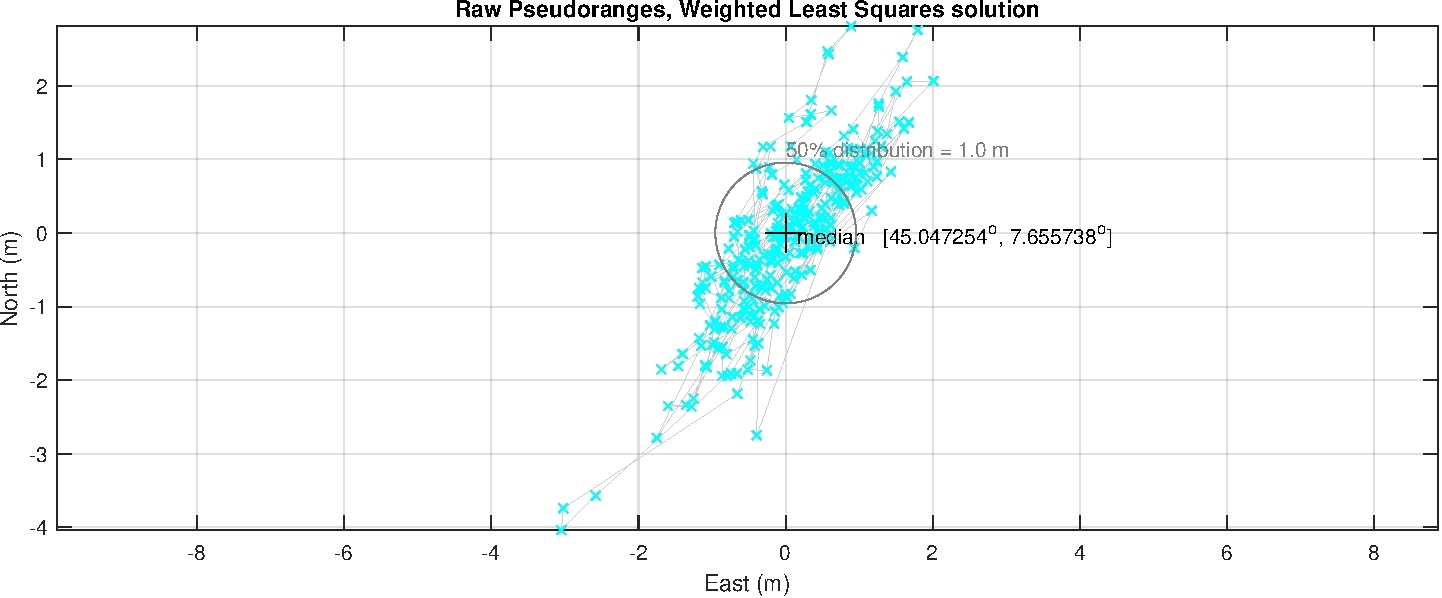
\includegraphics[width=1.00\linewidth]{images/pos_punto_3_precision.pdf}
        \caption{Positioning geoplot for logs collected in open-sky conditions (\ref{sec:opensky})}
        \label{fig:pos_punto_3_precision}
        \end{minipage}
    \hfill
    \begin{minipage}[b]{0.48\linewidth}
        \centering
        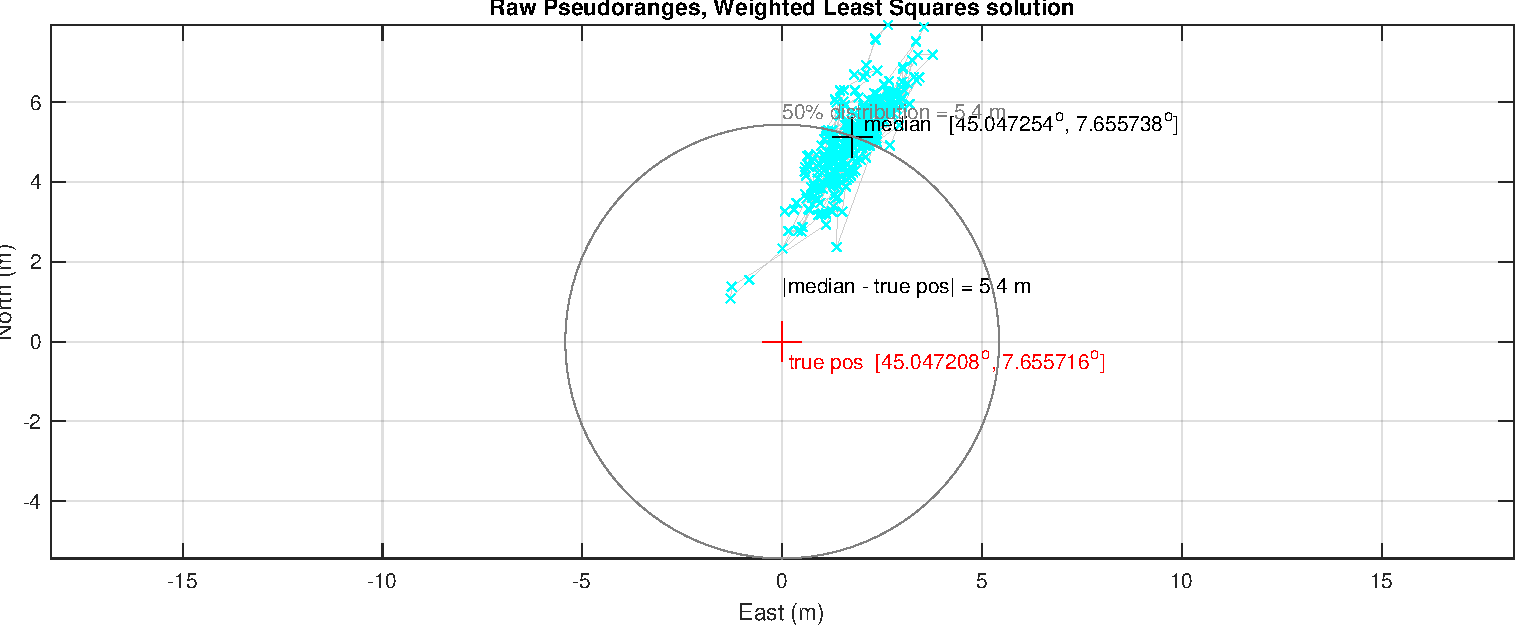
\includegraphics[width=1.00\linewidth]{images/pos_punto_3.pdf}
        \caption{Positioning geoplot for logs collected in open-sky conditions, correlated with true position (\ref{sec:opensky})}
        \label{fig:pos_punto_3}

    \end{minipage}
\end{figure}

\begin{figure}[H]
    \centering
    \begin{minipage}[b]{0.48\linewidth}
        \centering
        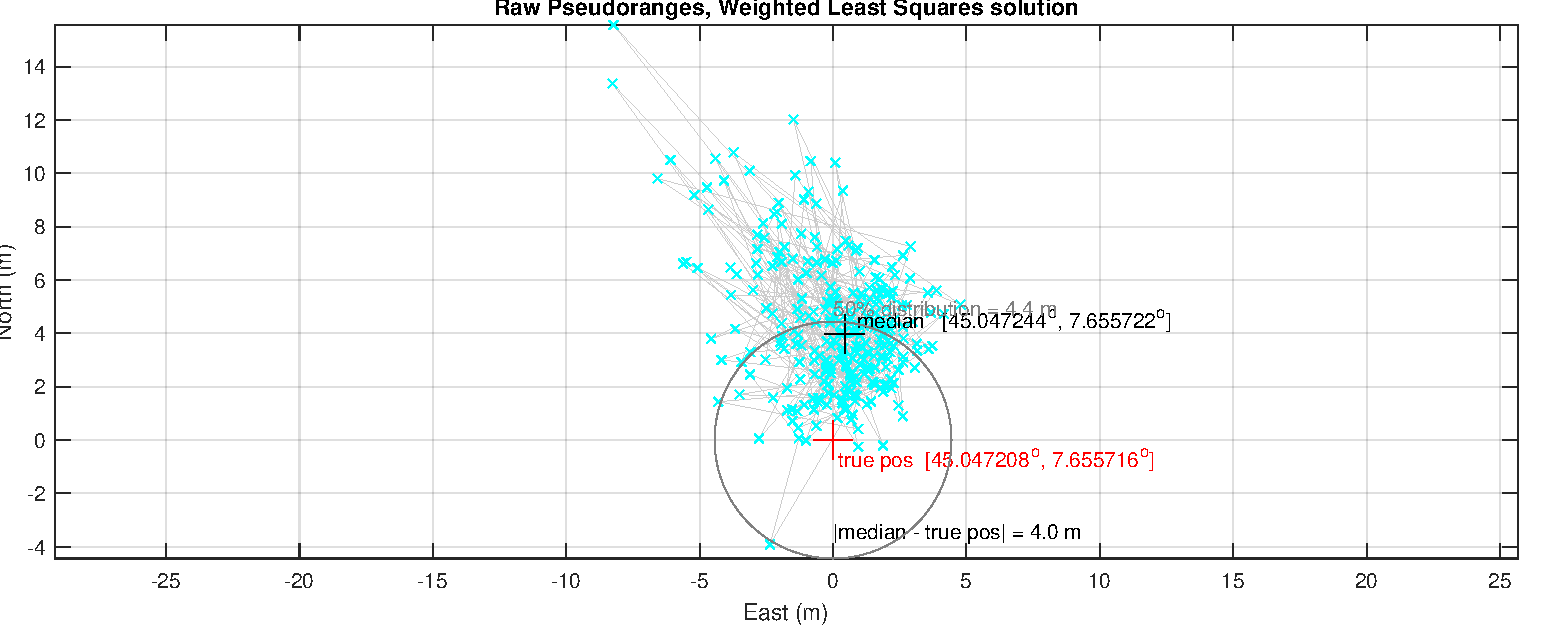
\includegraphics[width=1.00\linewidth]{images/carne_pos.pdf}
        \captionsetup{labelformat=empty}
        \caption{\textbf{Figure \ref{fig:carne_pos}:} Positioning geoplot for logs collected in the interference scenario (\ref{sec:opensky})}
        \end{minipage}
    \hfill
    \begin{minipage}[b]{0.48\linewidth}
        \centering
        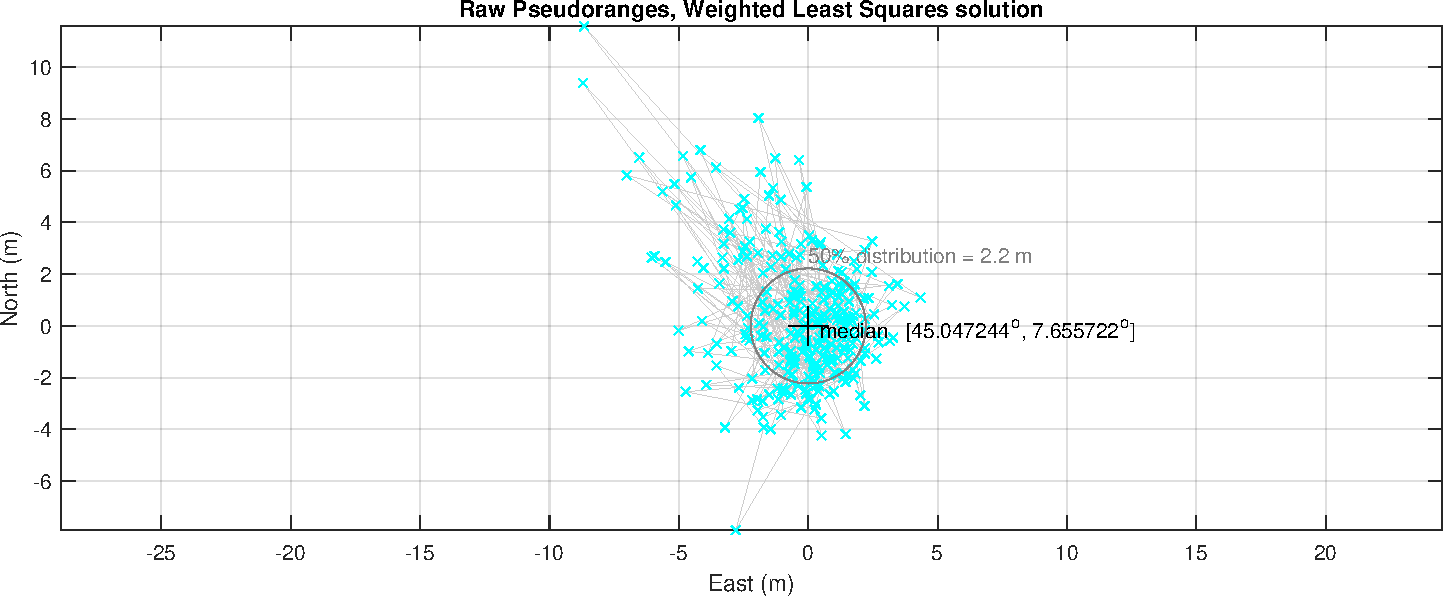
\includegraphics[width=1.00\linewidth]{images/carne_pos_precision.pdf}
        \caption{Positioning geoplot for logs collected in the interference scenario, correlated with true position (\ref{sec:opensky})}
        \label{fig:carne_pos_precision}

    \end{minipage}
\end{figure}


\begin{figure}[H]
    \centering
    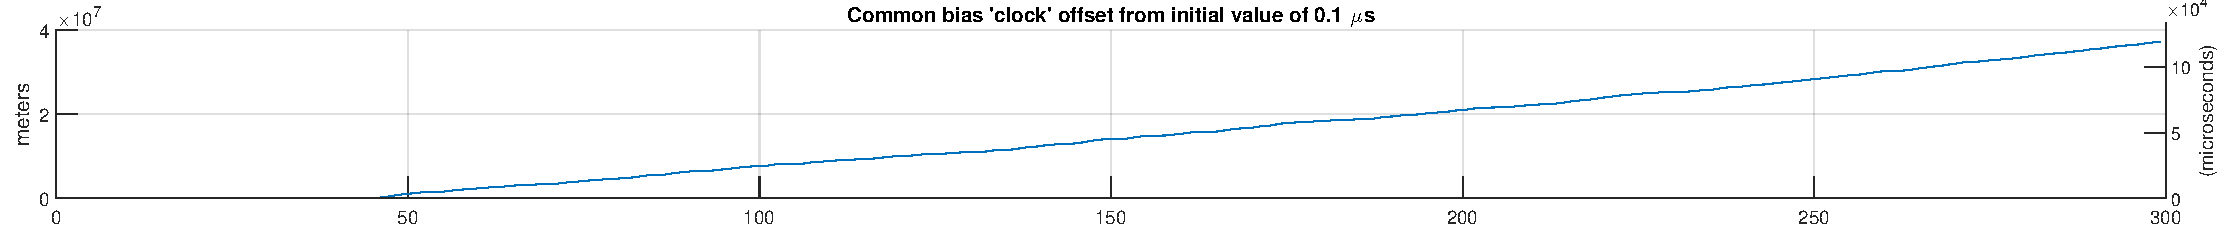
\includegraphics[width=0.95\linewidth]{images/discontinuity_bias_clock.pdf}
    \caption{Common bias clock offset in HW clock discontinuity} 
    \label{fig:discontinuity_bias_clock}
\end{figure}

\begin{figure}[H]
        \centering
        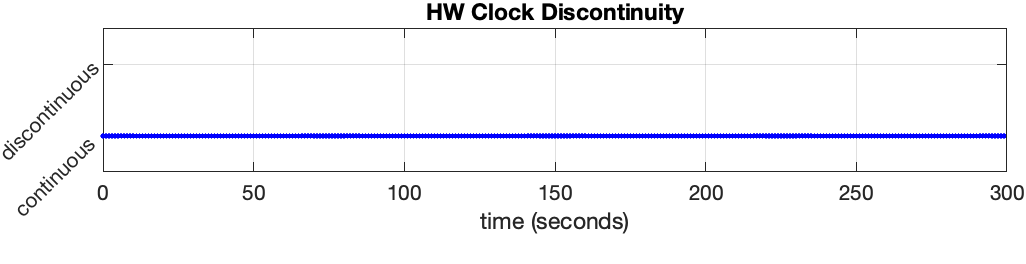
\includegraphics[width=0.85\linewidth]{images/continuity_gnss_log.png}
        \caption{Status of the GNSS hardware clock over time with GNSSLogger and GPSTest in parallel}
        \label{fig:GNSSLogger-continuity}
\end{figure}

\begin{figure}[H]
    \centering
    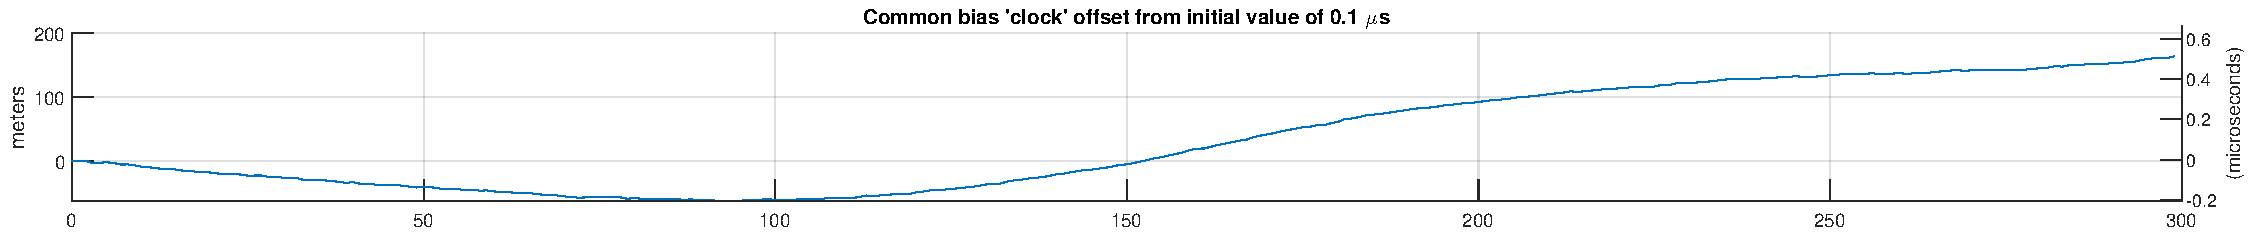
\includegraphics[width=0.95\linewidth]{images/continuity_bias_clock.pdf}
    \caption{Common bias clock offset in open-sky and HW clock continuity conditions (\ref{sec:opensky})} 
    \label{fig:continuity_bias_clock}
\end{figure}


\begin{figure}[H]
    \centering
    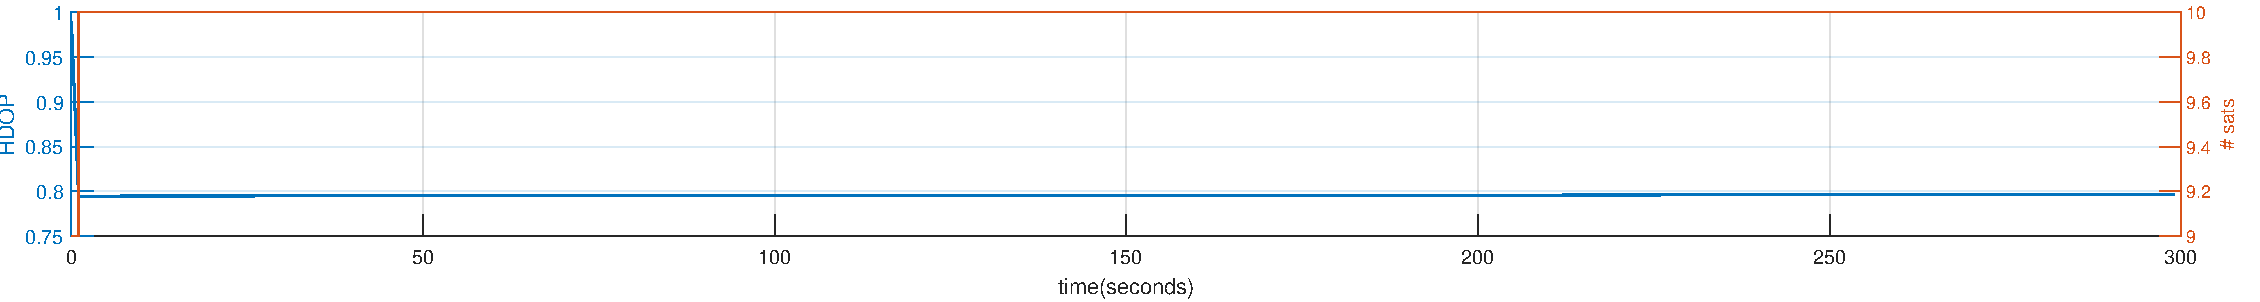
\includegraphics[width=1.00
    \linewidth]{images/hdop_punto_3.pdf}
    \caption{Horizontal diluition and number of satellites for logs collected in open-sky conditions (\ref{sec:opensky})}
    \label{fig:hdop_punto_3}
\end{figure}

\begin{figure}[H]
    \centering
    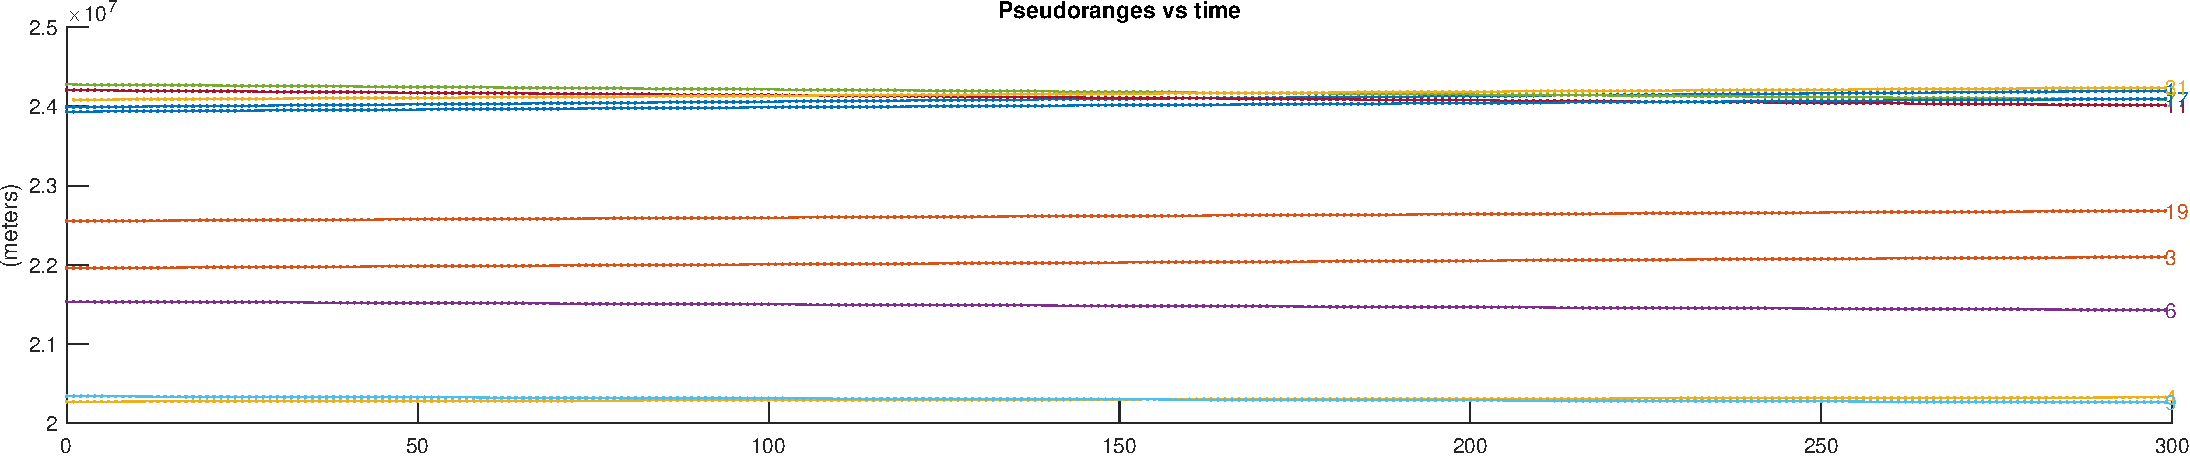
\includegraphics[width=1.00
    \linewidth]{images/punto3_pseudoranges.pdf}
    \caption{Pseudoranges vs. time for logs collected in open-sky conditions (\ref{sec:opensky})}
    \label{fig:pseudoranges_opensky}
\end{figure}

\begin{figure}[H]
    \centering
    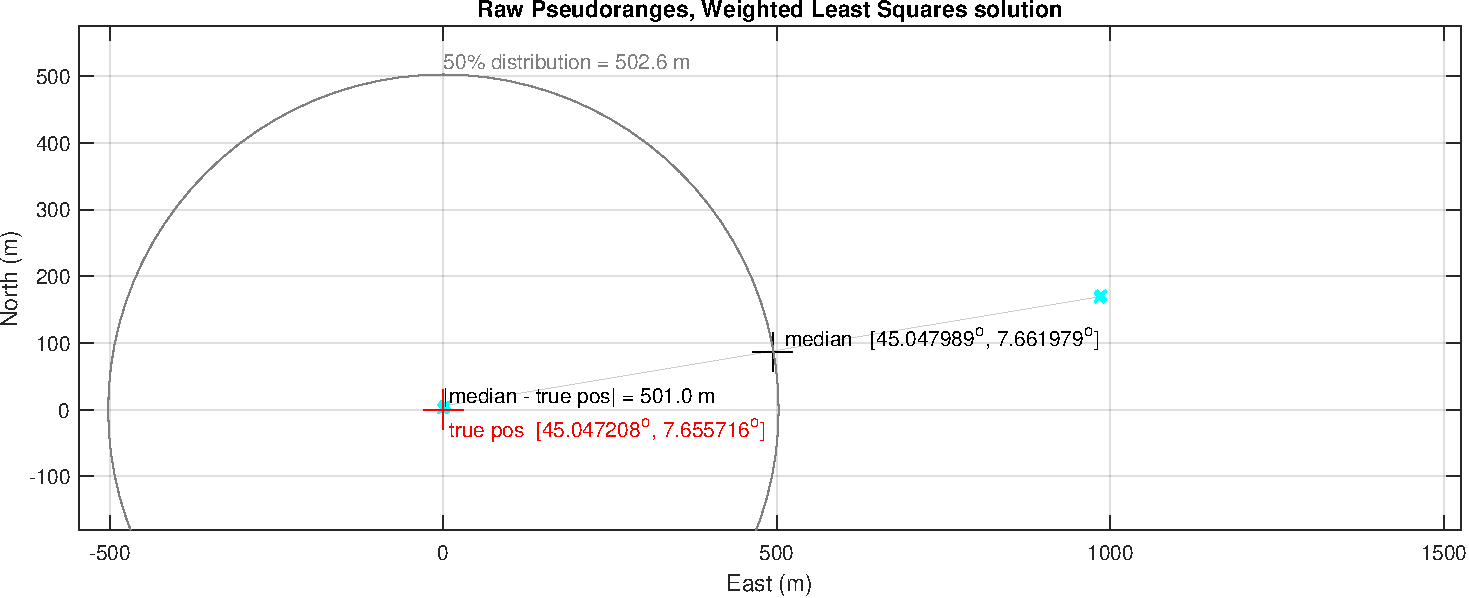
\includegraphics[width=1.00
    \linewidth]{images/pos_spoofed_no_delay.pdf}
    \caption{Positioning geoplot after applying spoofing to a location 1 Km from the real one, with no additional time delay used}
    \label{fig:pos_spoofed_no_delay}
\end{figure}

\begin{figure}[H]
    \centering
    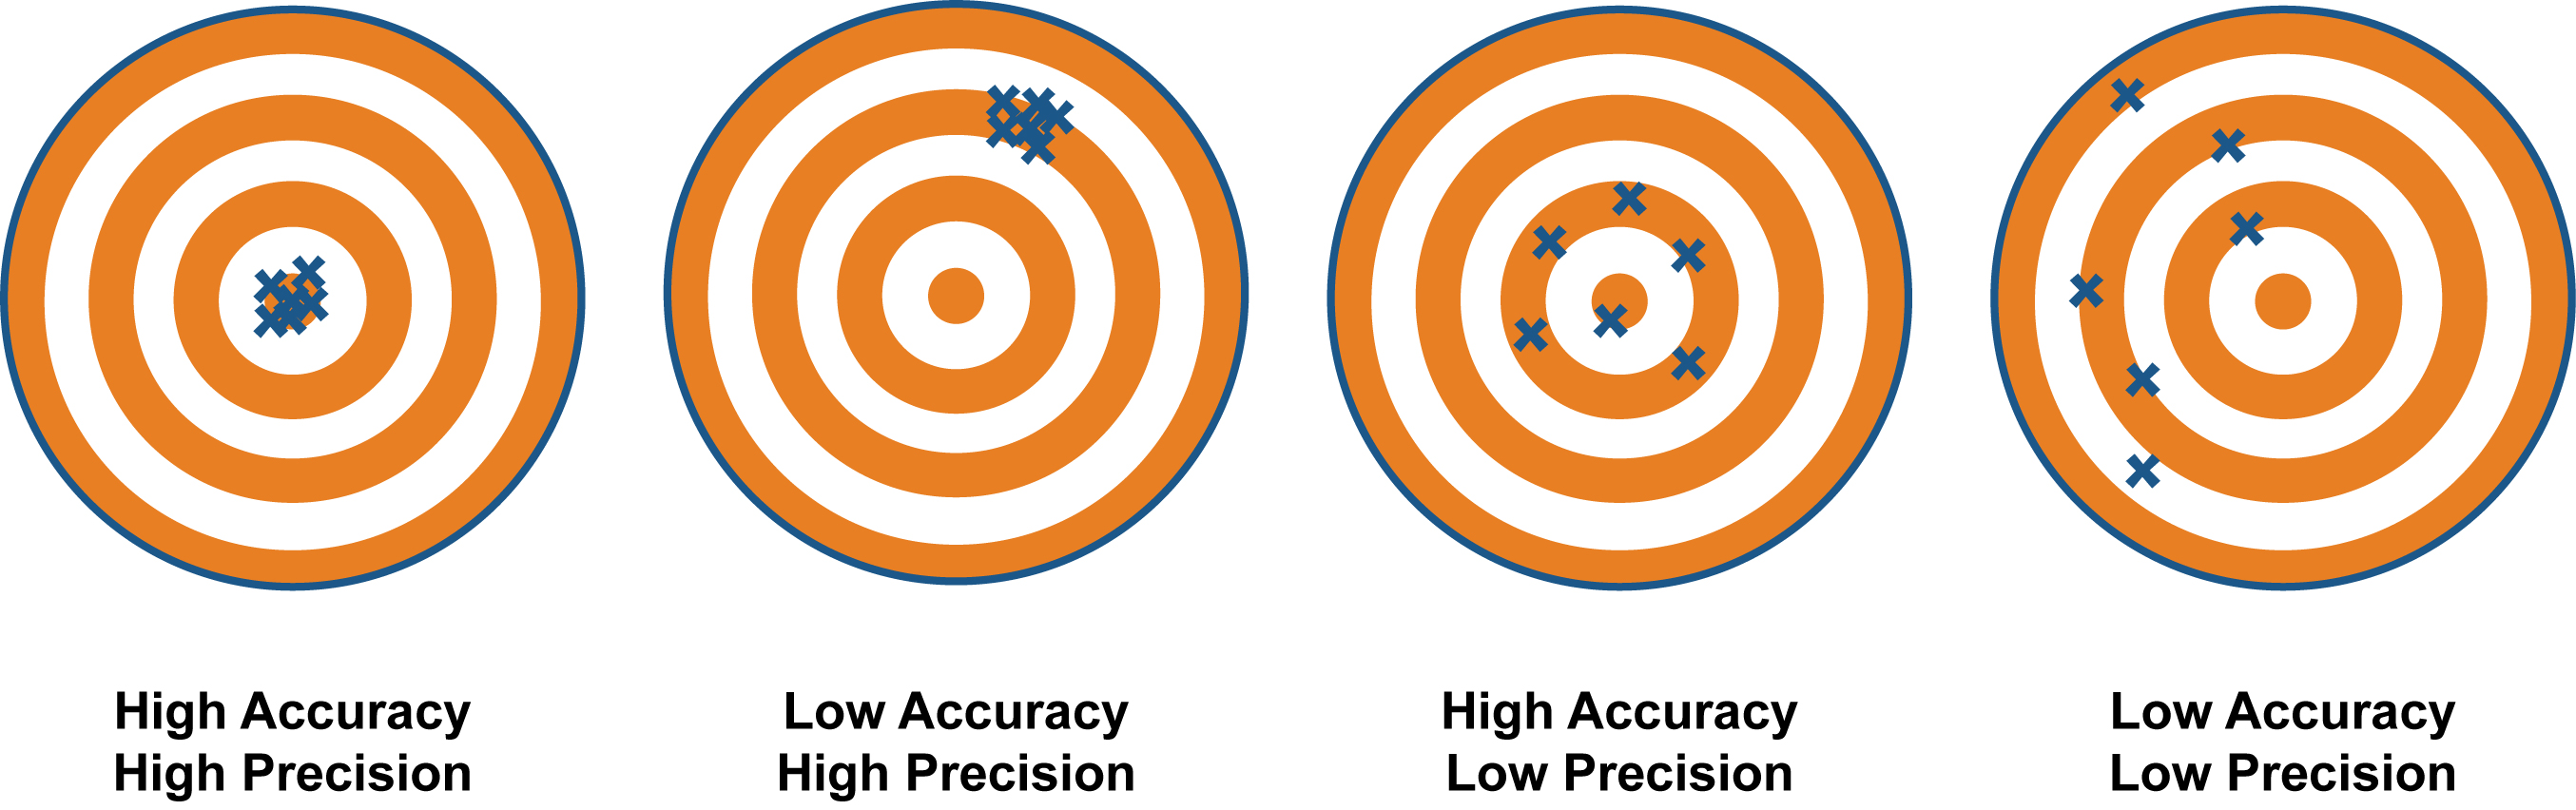
\includegraphics[width=0.50
    \linewidth]{images/Accuracy-vs-precision1.jpg}
    \caption{Accuracy vs. Precision}
    \label{fig:accPos}
\end{figure}

% \section{Appendix section title}
% \label{sec:underwater-comm}
% \colorbox{yellow}{Do we need this?}

% \begin{minted}[fontsize=\small, breaklines]{python}
% import subprocess
% import time
% import numpy as np
% import csv

% def run_iperf(name, server_ip, bind_ip, reverse, repetitions, pcap_fileNoExt, server_port, duration, udp, bitrate, app_buff_length):
% \end{minted}


\end{document}


%%% Local Variables:
%%% mode: latex
%%% TeX-master: t
%%% End:
